\documentclass[a4paper, openany, 12pt]{article}

%% подключаем стандарт библиографии
\bibliographystyle{gost71u}

%% для "Abstract" в классе book
% \newenvironment{abstract}{}{}
% \usepackage{abstract}

%% подключаем преамбулу: в ней содержится подключение всех необходимых пакетов
%% Работа с русским языком и шрифтами (XeLaTeX)
\usepackage{fontspec}
\defaultfontfeatures{Ligatures=TeX}
\setmainfont{Times New Roman}[
  Path=C:/Windows/Fonts/,
  UprightFont=times.ttf,
  BoldFont=timesbd.ttf,
  ItalicFont=timesi.ttf,
  BoldItalicFont=timesbi.ttf
]
\setsansfont{Times New Roman}[
  Path=C:/Windows/Fonts/,
  UprightFont=times.ttf,
  BoldFont=timesbd.ttf,
  ItalicFont=timesi.ttf,
  BoldItalicFont=timesbi.ttf
]
\setmonofont{Courier New}[
  Path=C:/Windows/Fonts/,
  UprightFont=cour.ttf,
  BoldFont=courbd.ttf,
  ItalicFont=couri.ttf,
  BoldItalicFont=courbi.ttf,
  Scale=MatchLowercase
]
\usepackage[russian]{babel}
\usepackage{microtype}
\usepackage{xurl}
\usepackage{fvextra}

% Перенос длинных латинских идентификаторов в русском тексте (XeLaTeX)
\XeTeXlinebreaklocale "en"
\XeTeXlinebreakskip = 0pt plus 3pt minus 1pt

\RecustomVerbatimEnvironment{verbatim}{Verbatim}{
  breaklines=true,
  breakanywhere=true,
  breaksymbol={},
  fontsize=\small
}

%% Пакеты для работы с математикой
\usepackage{amsmath,amsfonts,amssymb,amsthm,mathtools}
\usepackage{icomma}

%% Нумерация формул (опционально)
%\mathtoolsset{showonlyrefs=true}
%\usepackage{leqno}

%% Шрифты
\usepackage{euscript}
\usepackage{mathrsfs}

%% Некоторые полезные макросы для дебага
\makeatletter
\newcommand\thefontsize{The current font size is: \f@size pt}
\makeatother

%% Настройка размеров шрифтов
\makeatletter
\setlength{\headheight}{28pt}
\renewcommand\Huge{\@setfontsize\Huge{14pt}{10}}
\renewcommand\huge{\@setfontsize\huge{14pt}{10}}
\renewcommand\Large{\@setfontsize\Large{14pt}{10}}
\renewcommand\large{\@setfontsize\large{12pt}{10}}
\makeatother

%% Поля (геометрия страницы)
\usepackage[left=3cm,right=1.5cm,top=2cm,bottom=2cm,bindingoffset=0cm]{geometry}

%% Русские списки
\usepackage{enumitem}
\makeatletter
\AddEnumerateCounter{\asbuk}{\russian@alph}{щ}
\makeatother

%% Работа с картинками
\usepackage{caption}
\captionsetup{labelsep=endash}
\captionsetup[figure]{justification=centering}
\captionsetup[table]{justification=raggedright, singlelinecheck=false}
\addto\captionsrussian{\renewcommand{\figurename}{Рисунок}}
\usepackage{graphicx}
\graphicspath{{images/}{images2/}}
\setlength\fboxsep{3pt}
\setlength\fboxrule{1pt}
\usepackage{wrapfig}

%% Работа с таблицами
\usepackage{array,tabularx,tabulary,booktabs}
\usepackage{longtable}
\usepackage{multirow}
\usepackage{makecell}
\usepackage{hhline}

%% Красная строка
\setlength{\parindent}{1.25cm}
\emergencystretch=4em
\tolerance=4000
\pretolerance=1000
\AtBeginDocument{\hbadness=10000}

%% Интервалы (ГОСТ: полуторный межстрочный интервал)
\usepackage{setspace}
\onehalfspacing

%% Компактные вертикальные отступы вокруг плавающих объектов, подписей и списков
\setlength{\textfloatsep}{8pt plus 2pt minus 2pt}
\setlength{\floatsep}{8pt plus 2pt minus 2pt}
\setlength{\intextsep}{8pt plus 2pt minus 2pt}
\captionsetup{skip=4pt}
\setlist{topsep=3pt, itemsep=2pt, parsep=0pt}

%% Заголовки
\usepackage{titlesec}
\titleformat{\section}[block]
  {\normalfont\bfseries\fontsize{14pt}{16pt}\selectfont\centering}
  {\thesection}{1em}{}
\titleformat{\subsection}[block]
  {\normalfont\bfseries\fontsize{14pt}{16pt}\selectfont\centering}
  {\thesubsection}{1em}{}
\titlespacing*{\section}{0pt}{1.6ex plus .4ex minus .2ex}{1.0ex plus .2ex}
\titlespacing*{\subsection}{0pt}{1.3ex plus .3ex minus .2ex}{0.8ex plus .2ex}

%% TikZ
\usepackage{tikz}
\usetikzlibrary{graphs,graphs.standard}
\usetikzlibrary{positioning,arrows.meta,shapes.geometric,shapes.misc,fit,backgrounds,calc}

%% Цветовая палитра для схем
\usepackage{xcolor}
\definecolor{schemeBlue}{HTML}{2C5F8A}
\definecolor{schemeBlueLt}{HTML}{D6E6F2}
\definecolor{schemeGreen}{HTML}{2E7D5B}
\definecolor{schemeGreenLt}{HTML}{D5EFE2}
\definecolor{schemeOrange}{HTML}{C2611F}
\definecolor{schemeOrangeLt}{HTML}{FBE3D0}
\definecolor{schemeGray}{HTML}{4A4A4A}
\definecolor{schemeGrayLt}{HTML}{ECECEC}
\definecolor{schemeRed}{HTML}{B23A3A}

%% Верхний и нижний колонтитулы
\usepackage{fancyhdr}
\pagestyle{fancy}
\fancyhf{}
\fancyfoot[C]{\thepage}
\renewcommand{\headrulewidth}{0pt}
\renewcommand{\footrulewidth}{0pt}
\fancypagestyle{plain}{
  \fancyhf{}
  \fancyfoot[C]{\thepage}
  \renewcommand{\headrulewidth}{0pt}
  \renewcommand{\footrulewidth}{0pt}
}

%% Перенос знаков в формулах (по Львовскому)
\newcommand*{\hm}[1]{#1\nobreak\discretionary{}{\hbox{$\mathsurround=0pt #1$}}{}}

%% Дополнительно
\usepackage{float}
\usepackage{gensymb}
\usepackage{listings}
\let\monospacetext\texttt
% \texttt переопределён выше (переносы длинных путей и идентификаторов)
% Переменные текстом (не math-mode): корректный слой PDF для Антиплагиата
\newcommand{\kreq}{K\_req}
\newcommand{\kmin}{K\_min}
\newcommand{\aptimes}[1]{×#1}
\lstset{
basicstyle=\small\ttfamily,
columns=flexible,
breaklines=true
}

% Hyperref (для ссылок внутри pdf; hidelinks — меньше шума в текстовом слое)
\usepackage[hidelinks,unicode]{hyperref}
\urlstyle{same}
\def\UrlFont{\normalfont}
\def\UrlBreaks{\do\/\do-\do\_\do\.\do\ \do\:\do\;\do\=\do\~\do\(\do\)\do\[\do\]}

% Идентификаторы и пути — обычный текст (переносы: XeTeX linebreak + emergencystretch)
\DeclareRobustCommand{\texttt}[1]{%
  \ifmmode
    \text{\normalfont #1}%
  \else
    {\normalfont #1}%
  \fi
}

% Термин — определение (единый формат, без скачков description)
\newcommand{\defitem}[2]{%
  \par\smallskip\noindent\textbf{#1}~---~#2%
}

% Отступ перед первым абзацем в каждом разделе
\usepackage{indentfirst}

% Глубина нумерации и оглавления
\setcounter{secnumdepth}{2}
\setcounter{tocdepth}{2}


\begin{document}
    %% титульник убран для загрузки в ЛК (ЛК добавляет титул сам)
    % \input{include/title-page.tex}
    % \newpage

    \setcounter{page}{2}
    \fancyfoot[c]{\thepage}
    %% *надпись над верхним колонтитулом*
    %% в случае ненадобности можно удалить
    %% Колонтитул с названием рвёт связность текста в Антиплагиате — оставляем только номер страницы.
    % \fancyhead[L]{% Единое место для указания названия работы
Предобработка мешей для использования в ускоряющих структурах
}
    % \fancyhead[R]{}

    %% аннотация
    \begin{abstract}

    \begin{center}
        \large{% Единое место для указания названия работы
Предобработка мешей для использования в ускоряющих структурах
} \\
    \large\textit{Мусько Денис Владимирович} \\[1 cm]
    \end{center}

    Работа посвящена ускорению трассировки лучей в реальном времени за счёт
    предобработки геометрии перед подачей в структуру нижнего уровня (BLAS).
    Графический конвейер часто выделяет отдельный BLAS под каждый материал;
    если треугольники материала разбросаны по крупной модели, его AABB
    охватывает всю модель, а в TLAS возникают огромные перекрывающиеся
    инстансы, и луч вынужден пересекать почти все BLAS сцены.

    Цель --- разработать и оценить метод рантайм-предобработки, повышающий
    качество BLAS без визуальных потерь. Предложена глобальная
    пространственная кластеризация: треугольники всех материалов объединяются,
    сортируются по Morton-коду центроида и разбиваются на K компактных
    кластеров, каждый из которых регистрируется как отдельный BLAS с малым
    AABB. Метод работает на стороне CPU, не требует изменений драйвера и
    сохраняет попиксельную идентичность изображения.

    Метод реализован в семпле \texttt{testGI} движка DagorEngine. На «плохом»
    разбиении модели время \texttt{rtsm::do\_trace} падает в 8,6 раз
    (с 9,15 до 1,07~мс), на реалистичном --- в 2,7 раза
    (с 2,75 до 1,01~мс). Корректность подтверждена сравнением картин
    Acceleration Structure в Nsight Graphics. Рекомендуемый диапазон ---
    K от 64 до 128.


\end{abstract}

    \newpage

    %% содержание
    \tableofcontents{}
    \newpage

    % \fontsize{14}{16}\selectfont
    \section{Введение}
\label{sec:Chapter0} \index{Chapter0}

\subsection{Актуальность}

Трассировка лучей (ray tracing) в последнее десятилетие стала
основным алгоритмом физически корректного рендеринга и активно
проникает в реальное время благодаря появлению специализированных
аппаратных блоков NVIDIA RT~Cores и AMD Ray~Accelerators, а также
программных интерфейсов DirectX~Raytracing (DXR) и Vulkan
\texttt{KHR\_ray\_tracing}. Однако стоимость одного ray-primitive
теста растёт линейно с числом примитивов сцены, поэтому без
ускоряющей пространственной структуры данный подход
непригоден для интерактивных применений~\cite{paper}.

Стандартом де-факто для таких структур стала иерархия охватывающих
объёмов (Bounding~Volume~Hierarchy, BVH). При трассировке луч
обходит дерево BVH и отбрасывает поддеревья, AABB которых не
пересекается с лучом, что переводит сложность поиска ближайшего
пересечения в среднем к $O(\log n)$. Качество BVH принято измерять
поверхностно-площадной эвристикой (Surface Area Heuristic, SAH)~\cite{paper, ganestam16_splitting}:
\begin{equation}
    c(N) = c_T \sum_{N_i \in \text{Internal}} \frac{SA(N_i)}{SA(N)} + c_I \sum_{N_l \in \text{Leaf}} \frac{SA(N_l)}{SA(N)}\,|N_l|
\end{equation}
где:
\begin{itemize}
    \item $N$ --- корневой узел поддерева;
    \item $\text{Internal}$ и $\text{Leaf}$ --- множества внутренних (развилки дерева, хранящие AABB потомков) и листовых узлов (хранящие сами треугольники);
    \item $SA(X)$ --- площадь поверхности AABB узла $X$;
    \item $c_T$ и $c_I$ --- константные стоимости обхода узла и теста пересечения с треугольником;
    \item $|N_l|$ --- число треугольников в листе $N_l$.
\end{itemize}

Формула считает ожидаемую стоимость трассировки луча на основе геометрической вероятности: отношение площадей $SA(X) / SA(N)$ --- это шанс того, что луч, прошедший через $N$, пересечёт и вложенный узел $X$. При этом, если AABB дочерних узлов сильно перекрываются, их суммарная площадь увеличивается, лучу чаще приходится обходить обе ветви, и рендеринг становится дороже.

В современных графических приложениях BVH строится в два уровня:
\begin{itemize}
    \item \textbf{BLAS (Bottom-Level Acceleration Structure)} --- структуры нижнего уровня. Каждая из них содержит вершины и индексы треугольников отдельного меша или 3D-модели в локальной системе координат.
    \item \textbf{TLAS (Top-Level Acceleration Structure)} --- структура верхнего уровня. Она не содержит ассетов напрямую, а состоит из инстансов BLAS, расставленных по сцене с определёнными матрицами трансформаций (позиция, вращение, масштаб).
\end{itemize}
Такое разделение позволяет быстро обновлять сцену при движении объектов (достаточно перестроить только TLAS), не перестраивая тяжёлые BLAS для самих ассетов. Общая схема двухуровневой структуры и место, в котором возникает исследуемая проблема, показаны на приведённой ниже схеме.

\begin{figure}[h!]
\centering
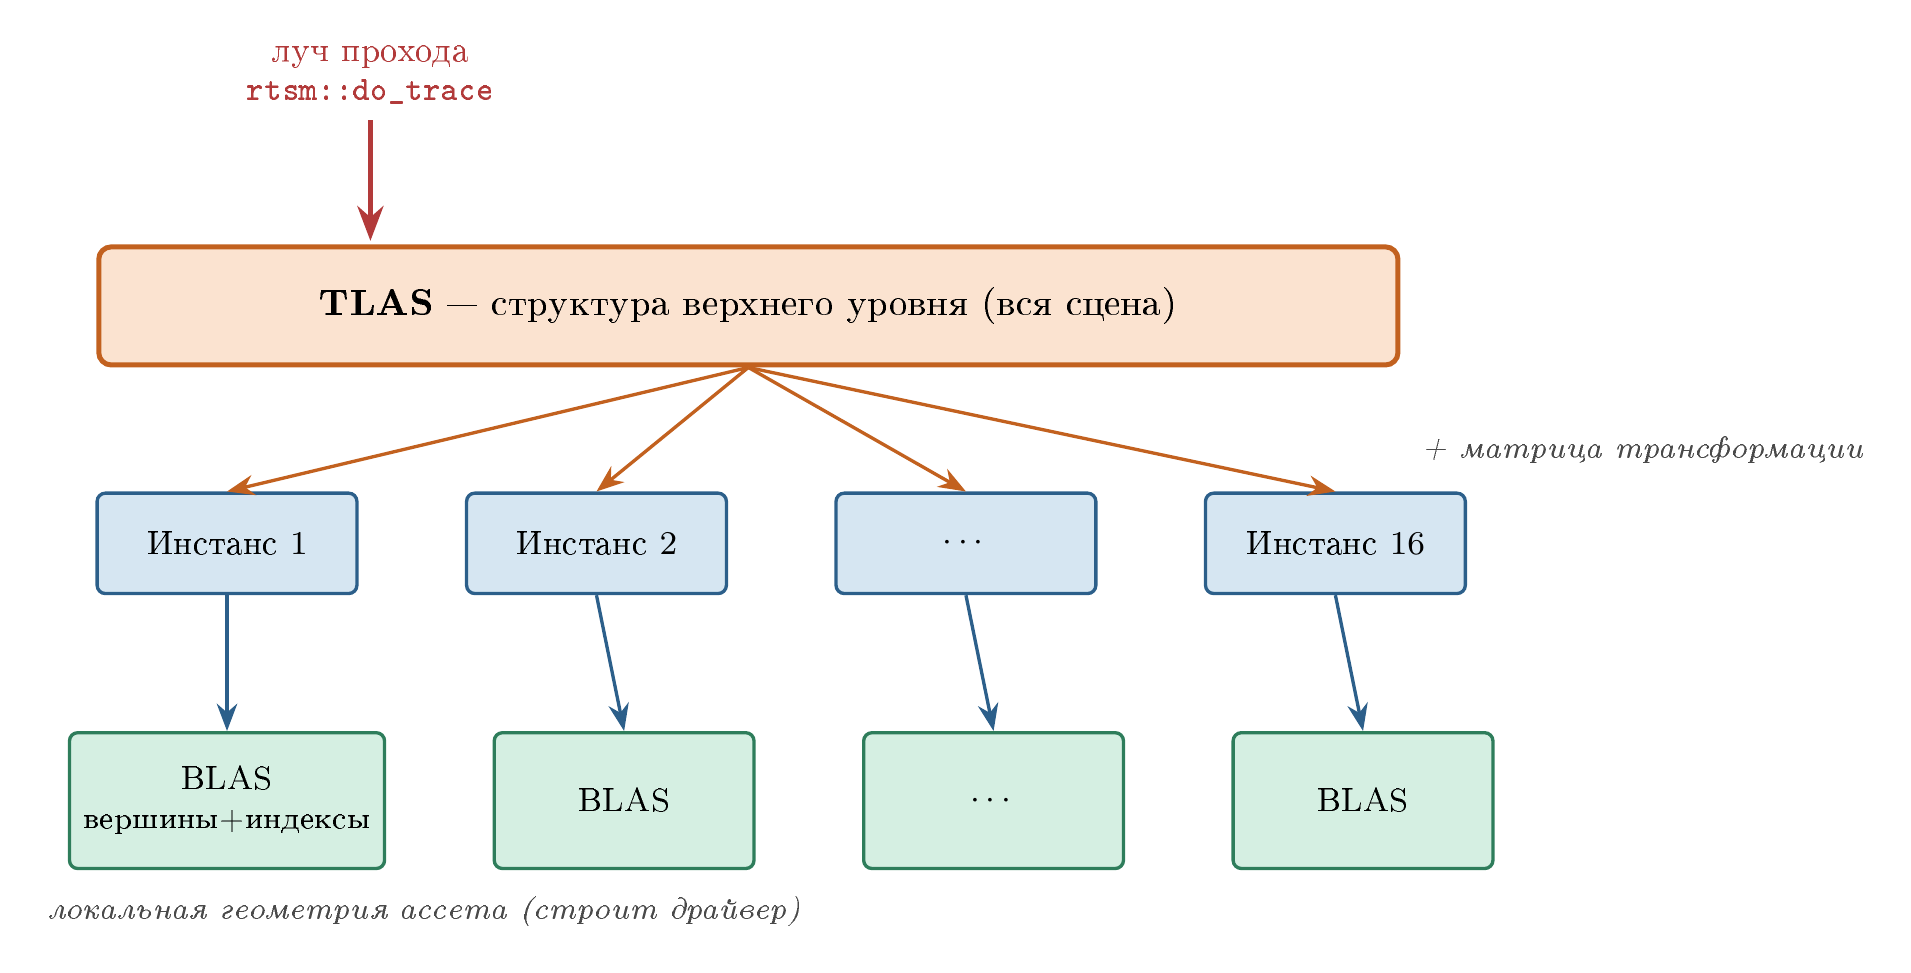
\includegraphics[width=0.82\textwidth]{diagrams/scheme_tlas_blas.png}
\caption{Двухуровневая структура ускорения в семпле \texttt{testGI}:
сцена из 16 инстансов модели порождает TLAS, листья которого ссылаются
на BLAS отдельных ассетов. Луч прохода \texttt{rtsm::do\_trace} сначала
обходит TLAS, затем спускается в BLAS. Именно качество BLAS и степень
перекрытия их AABB в TLAS определяют стоимость трассировки.}
\label{fig:arch_tlas_blas}
\end{figure}

На этом фоне построение BLAS, как правило, выполняется драйвером графического
вендора и недоступно для прямого вмешательства разработчиком: API
DXR/Vulkan~RT принимает на вход \emph{набор ассетов} (vertex
buffer + index buffer + диапазон), а внутреннюю стратегию построения
выбирает драйвер. Это означает, что основной канал влияния на
качество BLAS со стороны разработчика --- \textbf{предобработка
меша до его передачи билдеру}.

\subsection{Объект и предмет исследования}

\textbf{Объект исследования} --- процесс построения и обхода ускоряющих структур данных для аппаратной трассировки лучей в реальном времени.

\textbf{Предмет исследования} --- методы и алгоритмы пространственной кластеризации и предобработки ассетов трёхмерных моделей, направленные на повышение качества структур нижнего уровня и ускорение рендеринга.

\subsection{Ключевые понятия}

\defitem{BVH}{Bounding~Volume~Hierarchy. Двоичное дерево, в листьях
  которого хранятся примитивы сцены, а во внутренних узлах --
  AABB всех потомков.}
\defitem{AABB}{Axis-Aligned Bounding Box. Параллелепипед со сторонами,
  параллельными осям координат, содержащий поддерево примитивов.}
\defitem{BLAS / TLAS}{Bottom- и Top-Level Acceleration Structure --
  два уровня иерархии BVH в современных графических API (DXR / Vulkan~RT). BLAS хранит сами ассеты модели, а TLAS организует их экземпляры на сцене.}
\defitem{RElem}{Атомарная меш-структура исследуемого движка
  DagorEngine (\texttt{ShaderMesh::RElem}). Содержит ссылку на
  материал и непрерывный поддиапазон вершин/индексов общего
  буфера; одному \texttt{RElem} соответствует одна
  \texttt{RaytraceGeometryDescription} на входе
  билдера.}
\defitem{Morton-код}{Числовая характеристика 3D-точки, полученная
  чередованием битов её нормированных координат. Сортировка
  точек по Morton-коду эквивалентна обходу пространства по
  заполняющей кривой Z-order, что обеспечивает локальность
  соседних элементов в массиве.}
\defitem{SAH cost}{Поверхностно-площадная стоимость BVH;
  общепринятая офлайн-мера качества дерева,
  коррелирующая с реальным временем
  трассировки~\cite{paper}.}
\defitem{RTSM}{Ray~Traced~Shadow~Map. Подсистема трассировки теней
  в DagorEngine, выполняющая ray-cast от каждого пикселя экрана
  в сторону источника света; целевая нагрузка для измерения
  ускорения.}

\subsection{Постановочная гипотеза}

Графический конвейер часто выделяет отдельный меш-ассет и, соответственно, отдельный BLAS под каждый уникальный материал, например, дерево или металл. Если элементы такого материала разбросаны по всему объёму крупной модели, то AABB соответствующего BLAS будет сопоставим с размерами всей модели. В результате в TLAS возникает множество огромных и полностью перекрывающихся инстансов --- по одному на каждый материал. При сборке TLAS AABB его листовых узлов получаются огромными и сильно перекрывающимися друг с другом. При трассировке луча алгоритм обхода вынужден проверять пересечение со всеми этими крупными BLAS, что может существенно снижать производительность рендеринга.

Изложенное обосновывает следующую гипотезу работы: \emph{объединение всех треугольников модели с последующим разделением её на множество независимых, пространственно-компактных мини-ассетов, выполненное на стороне CPU до подачи данных в билдер, демонстрирует устойчивое снижение времени аппаратной GPU-трассировки лучей на сценах с таким типом ассетов.}

\subsection{Степень разработанности темы}

Проблема качества BVH активно исследуется: классические top-down SAH-билдеры,
HLBVH и SBVH повышают качество дерева при пространственно компактном входе,
однако в DXR/Vulkan~RT построение BLAS выполняется драйвером и недоступно
для модификации изнутри. Отдельные приёмы предобработки (Morton-reorder,
SAH pre-splitting) совместимы с API, но не устраняют перекрытия в TLAS,
возникающие при материальном разбиении крупных моделей. Промышленные
руководства NVIDIA и AMD рекомендуют вручную нарезать «жирные» ассеты,
не предлагая автоматизированного runtime-решения. Таким образом, автоматическая
пространственная кластеризация на входе вендорского билдера остаётся
малоосвоенной.

\subsection{Цель и задачи}

\textbf{Цель} --- разработать и экспериментально оценить алгоритм
рантайм-предобработки мешей, повышающий качество BLAS, построенного
вендорским билдером, и достичь измеримого ускорения трассировки
лучей в реальной сцене игрового движка без визуальных потерь.

\textbf{Задачи}:
\begin{enumerate}
    \item Провести обзор существующих подходов к улучшению качества
      BVH, оценить их применимость в
      условиях фиксированного DXR-pipeline.
    \item Изучить цепочку формирования BLAS в DagorEngine и
      определить точку, в которой возможна предобработка меша без
      модификации драйвера.
    \item Реализовать алгоритм глобальной пространственной кластеризации ассетов на
      стороне runtime: объединение всех треугольников модели в
      единый массив, сортировка по Morton-коду, разбиение на $K$
      пространственно-компактных кластеров с собственными
      vertex/index-буферами.
    \item Провести замер ускорения трассировки на сцене с
      «плохими» ассетами в семпле \texttt{testGI} и подтвердить
      визуальную корректность результата.
    \item Сформулировать ограничения метода и направления
      дальнейшей работы.
\end{enumerate}

\subsection{Методы исследования}

Для решения поставленных задач использованы следующие методы.
\textbf{Теоретический} --- обзор и сравнительный анализ подходов к построению
и улучшению BVH с позиции совместимости с DXR-pipeline; формализация входных данных, ограничений и
критериев оценки.
\textbf{Проектный} --- анализ цепочки формирования BLAS в DagorEngine,
выделение точки вмешательства и проектирование алгоритма глобальной
пространственной кластеризации.
\textbf{Экспериментальный} --- программная реализация метода в семпле
\texttt{testGI}, измерение медианного GPU-времени \texttt{rtsm::do\_trace}
и качественная проверка пространственной локализации BLAS в Nsight~Graphics. Выбор GPU-замера вместо офлайн-метрик SAH
обоснован тем, что в DXR реальная стоимость трассировки определяется
драйверо-специфичным билдером и аппаратным обходом.

\subsection{Научная новизна}

В отличие от классических подходов
HLBVH~\cite{HLBVH} и SBVH-presplitting~\cite{ganestam16_splitting},
работающих \emph{внутри} билдера BVH, предлагаемый метод оперирует
исключительно \emph{до} вызова вендорского BLAS-билдера, выполняется
на стороне runtime и явно учитывает специфический интерфейс DXR. Это позволяет получать ускорение, не имея
исходного кода драйвера и не модифицируя ассет-пайплайн движка.

\subsection{Практическая значимость}

Метод применим как опционально включаемый этап подготовки
динамических ассетов при инициализации BVH-контекста и не
требует переэкспорта ассетов. Он встраивается в существующий
рантайм-код движка без изменения формата хранения мешей, что
критично для проектов индустриального масштаба, использующих
большие массивы готовых ассетов.
 %% Введение
    \clearpage
    \section{Постановка задачи}
\label{sec:Chapter1} \index{Chapter1}

\subsection{Формальная модель входа}

Рассматривается \textbf{статическая трёхмерная сцена (или крупная модель)} $S$, готовая к загрузке в ускоряющие структуры для аппаратной трассировки (TLAS и BLAS). 

На уровне данных графического движка $S$ представляет собой набор из $R$ независимых геометрий (меш-ассетов или \texttt{RElem} в терминологии DagorEngine~\cite{dagorEngine}):
\begin{equation}
    S = \bigl(V,\; \{M_k\}_{k=1}^{R}\bigr),
\end{equation}
где
\begin{itemize}
    \item $V \in \mathbb{R}^{n_v \times 3}$ -- единый массив (буфер), содержащий пространственные 3D-координаты $n_v$ уникальных вершин. Этот массив может быть общим (разделяемым) для всей сцены/ассета;
    \item $M_k \subset \{1,\dots,n_v\}^3$ -- набор треугольников $k$-того меш-ассета (геометрии/материальной подгруппы). Каждый треугольник задаётся тройкой индексов, ссылающихся на координаты вершин в общем буфере $V$;
    \item $R$ -- общее число изначальных логических кусков геометрии (например, разделённых по материалам).
\end{itemize}

В пайплайнах игровых движков графические дизайнеры зачастую разделяют сложные объекты не по пространственному признаку, а по логическому или материальному. Например, могут выделить в отдельный меш-ассет $M_k$ все деревянные конструкции сложного здания или уровня. Геометрия может существовать в нескольких уровнях детализации (LOD), при этом для формирования структуры трассировки используется геометрия наивысшего качества.

\subsection{Модель построения BLAS}

При подготовке к аппаратному рейтрейсингу графический движок подаёт каждую геометрию $M_k$ в драйвер как независимую сущность. В соответствии с этим билдер драйвера воспринимает каждый $M_k$ как единое целое и строит для него \emph{свой собственный} отдельный BLAS:
\begin{equation}
    \mathcal{B}\bigl(M_k\bigr) \;\longmapsto\; T_k,
\end{equation}
где $T_k$ -- бинарное дерево BVH, полученное из внутреннего билдера драйвера $\mathcal{B}$. 

При добавлении в сцену каждый такой построенный BLAS $T_k$ регистрируется в структуре верхнего уровня (TLAS) в виде отдельного инстанса (листового узла). Таким образом, составная сцена $S$ представлена в TLAS набором из $R$ независимых инстансов.

\subsection{Гипотеза проблемы}

Проблема возникает из-за способа группировки треугольников внутри исходных $M_k$. Поскольку каждый отдельный BLAS строится для всего подмеша $M_k$ целиком, качество построенного дерева $T_k$ и размер его ограничивающего объёма (AABB) напрямую зависят от того, насколько компактен этот подмеш в пространстве.

Если $M_k$ представляет собой логическую материальную группу (например, все деревянные конструкции здания), то его треугольники разбросаны по всему объёму здания. В результате:
1. Корневой AABB этого BLAS $T_k$ раздувается до размеров всего здания.
2. Внутри самого дерева $T_k$ получаются сильно перекрывающиеся внутренние узлы, так как SAH-билдеру сложно разделить пространственно-разреженную геометрию на неперекрывающиеся компактные объёмы.

Наличие в $S$ множества подобных подмешей (выделенных под разные материалы: металл, бетон, стекло и т.д.) приводит к тому, что в листьях TLAS образуется набор из $R$ огромных инстансов. Они полностью перекрывают друг друга в пространстве. При трассировке луч вынужден проверять пересечение практически со всеми этими инстансами, что приводит к существенному росту ложных пересечений и может существенно снижать производительность рендеринга.

\subsection{Содержательная задача}

Построить отображение $\pi$, которое преобразует исходный набор «проблемных» разбросанных геометрий $\{M_k\}$ в новый набор из $K$ пространственно-компактных мини-ассетов $\{M'_j\}$:
\begin{equation}
    \pi:\ \bigl(V,\; \{M_k\}_{k=1}^{R}\bigr) \;\longmapsto\; \bigl(\{V'_j\},\; \{M'_j\}_{j=1}^{K}\bigr).
\end{equation}
Метод извлекает все треугольники исходной геометрии (забывая об их изначальном разделении по материалам) и перегруппировывает их в $K$ новых кластеров $\{M'_j\}$ исключительно на основе их пространственной близости. Каждый кластер $M'_j$ получает собственные буферы и регистрируется в движке как совершенно новая, независимая геометрия. Драйвер, в свою очередь, построит для каждого из них свой компактный BLAS.

Набор новых ассетов должен удовлетворять следующим условиям:
\begin{enumerate}
    \item \textbf{Визуальная эквивалентность}. Для любого направления
      обзора результирующий рендер совпадает с исходным попиксельно с точностью до численных ошибок при той
      же камере и той же реализации шейдеров. Достаточное условие:
      объединение треугольников всех новых ассетов $M'_j$ совпадает
      (как мульти-множество) с множеством треугольников исходной составной сцены $S$.
    \item \textbf{Пространственная локализация}. Физический размер каждого нового мини-ассета должен быть существенно меньше размера всей исходной сцены. Формально, отношение диагонали ограничивающего параллелепипеда ($\mathrm{diag}(\mathrm{AABB})$) нового ассета к диагонали всей исходной сцены должно быть ограничено:
      \[
          \dfrac{\mathrm{diag}(\mathrm{AABB}(M'_j))}{\mathrm{diag}\left(\bigcup_k \mathrm{AABB}(M_k)\right)} \;\le\; \tau,
      \]
      где $\tau \in (0, 1)$ -- желаемый коэффициент уменьшения габаритов. Это гарантирует, что новые инстансы будут компактными и не будут сильно перекрываться друг с другом.
    \item \textbf{Контракт DXR}. Каждый новый меш-ассет $M'_j$ удовлетворяет
      ограничениям интерфейса DXR-билдера: непрерывность
      vertex/index-буферов, число вершин $\le 65{,}535$ для
      16-битного индекса (Dagor использует
      \texttt{uint16\_t}), а также лимиту на число внутренних подмешей (geometry-описаний) внутри одного BLAS: $\le M_{\max}\!=\!32$.
    \item \textbf{Снижение реального времени трассировки}. За счёт устранения перекрытий в TLAS (и внутри самих деревьев BLAS), время
      \texttt{rtsm::do\_trace} после применения метода удовлетворяет
      $t_{after} \le t_{before}\cdot(1 - \alpha)$ с $\alpha > 0$,
      демонстрирующим устойчивое снижение в условиях фиксированной камеры и
      установившегося состояния денойзера.
\end{enumerate}

\subsection{Технические требования}

\begin{description}[leftmargin=1.3cm,style=nextline]
\item[Платформа] Windows 10/11~x64, DirectX~12, DXR Tier 1.1,
  GPU NVIDIA Turing+ или AMD RDNA2+. Эталонная конфигурация
  замеров -- GeForce RTX-класса с поддержкой
  hardware-traversal.
\item[Окружение] DagorEngine, семпл \texttt{testGI}. Семпл
  поддерживает прямую загрузку моделей в \texttt{.dag}-формате
  через сценарии и обладает встроенным GPU-профайлером с
  таймингами по подсистемам.
\item[Целевая сцена] Модель \href{https://sketchfab.com/3d-models/house-ko-bulon-don-urak-lawoi-village-thailand-bc53e24d35a9439cac420cf530e7de3f}{\texttt{House, Ko Bulon Don Urak Lawoi Village, Thailand}} -- созданный
  специально для эксперимента «плохой» вариант жилого дома:
  $\sim 1{,}2\!\cdot\!10^6$ треугольников, $\sim 10$ материальных
  групп, геометрически разнесённых по всему объёму модели; в
  сцене размещены $N\!=\!16$ инстансов.
\item[Метрики измерения] (а) медианное время GPU-трассировки теней
  \texttt{rtsm::do\_trace}, измеренное через встроенный
  GPU-профайлер DagorEngine; (б) визуальная картина
  Acceleration-Structure в Nsight~Graphics с раскраской по
  индексу BLAS-инстанса для оценки качества пространственной
  локализации; (в) визуальное сравнение качества теней до и
  после оптимизации в финальном изображении.
\item[Аппаратное ограничение DXR Tier 1.1] Index-буферы BLAS в
  Dagor выделяются как \texttt{uint16\_t}, что ограничивает число
  вершин на одну BLAS-geometry значением $2^{16}-1$ и, при
  отсутствии sharing-а вершин, число треугольников значением
  $\lfloor (2^{16}-1)/3 \rfloor = 21\,845$. Метод обязан
  учитывать это ограничение.
\end{description}

\subsection{Критерии приёмки}

Работа считается выполненной успешно, если выполнено каждое из:

\begin{enumerate}
    \item Реализован метод пространственной кластеризации ассетов как
      опциональный режим инициализации BVH для динамических
      моделей в семпле \texttt{testGI}, включаемый из
      \texttt{settings.blk}; собирается штатным
      jam-скриптом DagorEngine.
    \item На модели \href{https://sketchfab.com/3d-models/house-ko-bulon-don-urak-lawoi-village-thailand-bc53e24d35a9439cac420cf530e7de3f}{\texttt{House, Ko Bulon Don Urak Lawoi Village, Thailand}} (16 инстансов в сцене)
      зафиксировано снижение медианного времени
      \texttt{rtsm::do\_trace} не менее чем в $2$ раза по
      сравнению с baseline-режимом без предобработки.
    \item Визуальная картина Acceleration-Structure в
      Nsight~Graphics с раскраской по индексу инстанса
      демонстрирует пространственно-связные области (а не
      «шумовую» картину перекрытий), подтверждая
      пространственную локализацию BLAS-кластеров.
    \item Сцена после применения метода визуально неотличима от
      сцены до его применения: тени, освещение и
      раскраска ассетов совпадают.
\end{enumerate}
 %% Постановка задачи
    \clearpage
    \section{Обзор существующих решений}
\label{sec:Chapter2} \index{Chapter2}

В разделе рассматриваются подходы к улучшению качества BVH. Для этого систематизация ведётся по двум осям: (i)~уровень
вмешательства в pipeline (внутрь билдера, на входе билдера, поверх
готового BVH) и (ii)~применимость в условиях, диктуемых
DXR/Vulkan~RT API. Для каждого подхода критически оценивается,
насколько он удовлетворяет ограничениям, сформулированным в
постановке задачи: неизменность кода
вендорского билдера, сохранение визуальной эквивалентности,
аппаратные лимиты на 16-битные индексы и число
geometry-описаний на BLAS.

\subsection{Классические top-down SAH-билдеры}

Поверхностно-площадная эвристика SAH
была введена Goldsmith и Salmon в 1987~г.~\cite{goldsmith1987} и
формализована для контекста ray-tracing-обхода
MacDonald и Booth в 1990~г.~\cite{macdonald1990}. SAH постулирует,
что вероятность попадания случайного луча в узел $X$ оценивается
отношением площадей поверхности,
$P(\text{hit}\,X)\!\approx\!SA(X)/SA(\text{root})$,
откуда выводится ожидаемая стоимость обхода всего дерева.

Top-down SAH-билдер на каждом узле перебирает кандидатов разбиения и выбирает $\arg\min$
SAH-стоимости. Точный перебор дорог на больших наборах примитивов.
Wald~\cite{wald2007} показал, что достаточно вдоль каждой оси
пространство делить на $16$~равных интервалов, примитивы
распределяются по ним, а лучшая плоскость разбиения выбирается среди
границ этих интервалов. Такой вариант работает за $O(n\log n)$ и даёт качество BVH,
отличающееся от варианта полного перебора менее чем на $1\,\%$, поэтому стал
стандартом в индустрии.

\textit{Соответствие задаче.} Этот подход --- \emph{внутренний} алгоритм
билдера. В DXR/Vulkan~RT он работает внутри драйвера, и для
разработчика доступа к нему нет. При этом любая SAH-оптимизация внутри
билдера улучшает результат лишь в рамках заданного входа: если
поданный на вход материальный подмеш имеет AABB размером со всю сцену, SAH-разбиение внутри него не
может предотвратить появление огромного BLAS, который в дальнейшем приведёт к перекрытиям в TLAS.

\subsection{HLBVH и LBVH: параллельная сборка по Morton-кривой}

Lauterbach и др. предложили LBVH (Linear~BVH): кодирование
центроидов примитивов 30-битным Morton-кодом, радикс-сортировка по
этому коду и рекурсивное построение дерева по битам ключа.
Pantaleoni и Luebke расширили подход до HLBVH~\cite{HLBVH},
реализовав параллельную постройку BVH для динамических ассетов
на GPU.

Идея Morton-сортировки используется и независимо от LBVH:
предварительная перестановка примитивов по Z-кривой
улучшает локальность
доступа в кэше и обычно даёт билдеру более стабильное разбиение. Это поведение закреплено как baseline-приём,
упоминаемый в практических руководствах
NVIDIA~\cite{nvOptMesh} и AMD~\cite{rraManual}.

\textit{Соответствие задаче.} HLBVH как замена вендорского билдера
не применим: для DXR/Vulkan-сцен дерево обязан построить драйвер.
Однако \emph{глобальная Morton-перестановка примитивов} на стадии,
предшествующей вызову билдера, полностью совместима с
DXR-контрактом, и именно этот приём используется в
настоящей работе как один из двух обязательных шагов
предлагаемого алгоритма: после
объединения треугольников всех материальных групп они
сортируются по Morton-коду центроида перед разбиением на
кластеры.

\subsection{SBVH и SAH-guided pre-splitting}

Параллельно линии классических билдеров развивалась идея ослабления
требования «один треугольник --- один лист». Stich и
др.~\cite{stich2009} (метод SBVH) показали, что разрешение
разрезать треугольник на несколько ссылок
повышает качество дерева на 10--30\,\% по SAH-стоимости при
умеренном раздувании числа ссылок. Ganestam и
Doggett~\cite{ganestam16_splitting} перенесли эту идею на стадию
\emph{пре-разрезания} больших треугольников до запуска top-down
билдера, что ускоряет последующую постройку и сохраняет
SBVH-качество.

\textit{Соответствие задаче.} Обе работы атакуют ту же
фундаментальную проблему --- большой AABB примитива, портящий
верхние узлы дерева, --- но на уровне отдельных треугольников. SBVH
встраивается в билдер и поэтому в DXR-сцене недоступен;
pre-splitting Ganestam--Doggett в принципе реализуем на стороне
CPU, однако он кратно увеличивает число треугольников меша, что в
условиях многократного использования ассета (рендер-проход, тени,
GI и т.\,п.) даёт значительную нагрузку на остальной pipeline.
Предлагаемый в настоящей работе подход концептуально близок к
pre-splitting на уровне идеи «компактизация на входе билдера», но
оперирует не отдельными треугольниками, а \emph{целыми крупными ассетами}:
исходный меш не разбивается на части внутри одного BLAS, а перегруппировывается
по пространственной близости в независимые мини-ассеты, и тем самым решает проблему перекрытий в TLAS.

\subsection{Метрики качества BVH}

Стандартная SAH-стоимость удобна, но является лишь \emph{прокси}
для реального времени трассировки. Aila, Karras и
Laine~\cite{ailaKarrasLaine2013} провели систематический анализ
корреляции офлайн-метрик с GPU-измерениями и показали:
(i)~на 20+ тестовых сценах коэффициент детерминации SAH cost
против реального времени \texttt{DispatchRays} составил
$R^2\!\approx\!0.85$;
(ii)~альтернативная метрика EPO (Expected~Path~Overlap) улучшает
корреляцию, но вычислительно дороже ($O(n^2)$ в худшем случае);
(iii)~кэш-эффекты и SIMD-ширина дают расхождение SAH-время до
15\,\% на сценах с регулярной структурой.

Karras и Aila~\cite{karras2013} также показали, что для
GPU-friendly~BVH важна не только SAH-стоимость, но и
сбалансированность дерева; несбалансированные SBVH-деревья могут
уступать сбалансированным LBVH-деревьям при одинаковой
SAH-стоимости.

\textit{Соответствие задаче.} Поскольку в DXR/Vulkan-сцене дерево
строится драйвером и реальная стоимость может зависеть от
драйверо-специфичных эвристик, в настоящей работе в качестве
основной метрики выбрано \emph{измеренное GPU-время} основного
прохода трассировки теней \texttt{rtsm::do\_trace}. Эта метрика
непосредственно отражает практический эффект оптимизации и не
зависит от выбранной офлайн-метрики; SAH cost упоминается лишь
как теоретическое объяснение причины ускорения.

\subsection{Альтернативные ускоряющие структуры}

Помимо BVH рассматриваются и альтернативные подходы. Aman и
др.~\cite{tetra2021} предложили компактное представление сцены на
основе тетраэдрализации, дающее меньший объём данных и линейную
сложность поиска ближайшего пересечения для протяжённых лучей.
KD-деревья и uniform~grid традиционно используются в
офлайн-рендерах. NVIDIA отдельно использует \emph{rebraiding}
TLAS-инстансов для динамической перестройки верхних
уровней~\cite{nvOptMesh}.

\textit{Соответствие задаче.} Все альтернативы предполагают замену
ускоряющей структуры целиком, что невозможно в условиях
фиксированного DXR-pipeline. Они рассматриваются как ориентиры для
понимания нижней границы возможной стоимости трассировки, но не
как конкуренты предлагаемого метода.

\subsection{Промышленные руководства и анализаторы}

NVIDIA в техническом руководстве~\cite{nvOptMesh} прямо рекомендует
разработчикам ассетов: (i)~избегать ассетов с диагональю
AABB, сопоставимой с размером всей сцены; (ii)~разрезать «жирные»
ассеты вручную в DCC-инструментах; (iii)~контролировать число
geometry-описаний на BLAS, желательно не более 16--32. AMD в
руководстве к RRA~\cite{rraManual} описывает аналогичный набор
рекомендаций и предоставляет инструмент для визуализации
SAH-стоимости и overlap-а во внутренних узлах BLAS непосредственно
из захвата GPU-памяти.

Спецификация DXR~\cite{dxrSpec} фиксирует контракт интерфейса:
поля \texttt{geometry\_index} и \texttt{primitive\_index} должны
оставаться стабильными при обходе и в hit-шейдере; диапазон
индексов одной \texttt{GeometryDesc} является \emph{непрерывным}. Это формальное
обоснование того, почему драйвер не может «разрезать» большую
geometry самостоятельно.

\textit{Соответствие задаче.} Эти руководства подтверждают практическую
актуальность проблемы, описанной в постановке. Однако они
оставляют выполнение рекомендаций за разработчиком ассетов и не
предлагают автоматизированного инструмента, работающего на
стороне runtime игрового движка. Настоящая работа закрывает эту
нишу: предлагается алгоритм и его реализация, которые выполняют
рекомендации NVIDIA автоматически при инициализации BVH-контекста
без вмешательства в ассет-пайплайн.

\subsection{Сводное сравнение}

В сводной таблице сведены ключевые свойства
рассмотренных подходов с позиции ограничений настоящей работы.

\begin{table}[H]
\centering
\caption{Сравнение подходов по совместимости с DXR-pipeline}
\label{tab:related_work}
\small
\begin{tabular}{lccc}
\hline
\textbf{Подход} & \textbf{Уровень} & \textbf{Совместим} & \textbf{Решает перекрытия} \\
& \textbf{вмешательства} & \textbf{с DXR} & \textbf{в TLAS} \\
\hline
Top-down SAH binner~\cite{wald2007} & внутри билдера & --- & частично \\
HLBVH~\cite{HLBVH} & замена билдера & нет & нет \\
Morton-reorder & вход билдера & да & нет \\
SBVH~\cite{stich2009} & внутри билдера & --- & да \\
SAH pre-split~\cite{ganestam16_splitting} & вход билдера & да$^*$ & да \\
Tetra-AS~\cite{tetra2021} & замена структуры & нет & --- \\
\textbf{Глобальная пространственная} & \textbf{вход билдера} & \textbf{да} & \textbf{да} \\
\textbf{кластеризация (наш)} & & & \\
\hline
\end{tabular}

\vspace{0.5em}
\raggedright\footnotesize
$^*$~требует дисциплины: pre-split может вылезти за лимит числа
геометрий или 16-битного индекса, если применяется к большим
группам без учёта аппаратных ограничений.
\end{table}

\subsection{Выводы по обзору}

\begin{enumerate}
    \item Существующие алгоритмы построения BVH (top-down
      SAH binner, HLBVH, SBVH) показывают, что классические
      эвристики хорошо справляются с улучшением дерева,
      \emph{если} на вход подан пространственно компактный
      набор примитивов.
    \item Реальный DXR/Vulkan-pipeline ставит билдер в условия
      чёрного ящика и фиксирует контракт непрерывности
      индекс-диапазонов и формат 16-битных индексов. Любое
      решение, требующее модификации внутри билдера, этим
      ограничениям не удовлетворяет.
    \item Доступная разработчику зона вмешательства --- стадия до
      подачи в билдер. На этой стадии существуют отдельные приёмы
      (Morton-reorder, pre-splitting), но ни один из них не
      закрывает сценарий «отдельные материальные подмеши имеют размер всей сцены, вызывая огромные перекрытия в TLAS» при
      сохранении контракта DXR.
    \item Все упомянутые работы оценивают результат либо
      SAH-стоимостью, либо время-симулятором, но не на реальном
      production-движке. В настоящей работе оценка ведётся
      непосредственно по GPU-времени трассировки теней в
      работающем семпле DagorEngine, что повышает достоверность
      результата.
\end{enumerate}

Эти выводы определяют как цель алгоритмической части работы
при описании алгоритма, так и форму экспериментальной
валидации.
 %% Обзор существующих решений
    \clearpage
    \section{Исследование и построение решения задачи}
\label{sec:Chapter3} \index{Chapter3}

В разделе из общей содержательной задачи постановки
последовательно выделяются подзадачи, и для каждой из них строится
решение. При этом на каждом шаге фиксируются принятые проектные решения и
обоснование выбора.

\subsection{Декомпозиция задачи}

Поставленная задача --- построить отображение
$\pi: \{M_k\} \mapsto \{M'_j\}$ --- разбита на следующие
подзадачи:
\begin{enumerate}
    \item \textbf{Pipeline формирования BLAS для динамических
      ассетов в DagorEngine.} Без точного знания цепочки
      \texttt{mesh}, \texttt{geometry-array}, \texttt{BLAS}
      невозможно определить, какое представление меша менять
      и в какой момент времени.
    \item \textbf{Алгоритм объединения и переразбиения
      треугольников модели.} Должен сохранять множество
      треугольников, перегруппировывать их по пространственной
      близости и удовлетворять аппаратным ограничениям DXR
      (16-битный индекс, лимит числа геометрий на BLAS).
    \item \textbf{Способ валидации гипотезы.} Необходимо
      экспериментально подтвердить, что метод даёт реальное
      ускорение GPU-трассировки в работающем семпле движка.
\end{enumerate}

Подзадачи решаются последовательно в
подразделах ниже.

\subsection{Pipeline формирования BLAS в DagorEngine}
\label{ssec:p1}

Исследование исходного кода DagorEngine~\cite{dagorEngine} показывает,
что при подготовке BLAS для динамической модели выполняется следующая
цепочка преобразований:

\begin{equation}
\begin{split}
&\underbrace{\texttt{DynamicRenderableSceneLodsResource}}_{\text{ресурс модели}} \\
&\quad\;\to\; \underbrace{\texttt{ShaderMesh::RElem[]}}_{\text{меш-уровень}} \\
&\quad\;\to\; \underbrace{\texttt{RaytraceGeometryDescription[]}}_{\text{DXR-вход}} \\
&\quad\;\to\; \underbrace{\mathcal{B}}_{\text{драйвер}} \;\to\; \underbrace{T}_{\text{BLAS}}.
\end{split}
\label{eq:pipeline}
\end{equation}

\noindent
\textbf{(1) \texttt{DynamicRenderableSceneLodsResource}}~---~ресурс
динамической модели в Dagor; содержит несколько уровней детализации, каждый из
которых --- набор \texttt{ShaderMesh}. Для построения BLAS
используется наивысший уровень.

\noindent
\textbf{(2) \texttt{RElem}}~---~атомарная меш-структура графического движка. Содержит
указатель на материал, ссылку на разделяемый вершинный буфер
\texttt{vertexData} и диапазоны \texttt{(sv, numv, si, numf,
baseVertex)}. Один \texttt{RElem}~=~непрерывный поддиапазон
индексов с единой шейдер-материальной атрибуцией.

\noindent
\textbf{(3) \texttt{RaytraceGeometryDescription}}~---~DXR-совместимая
структура.
Массив таких структур и является \emph{основным входом}
вендорского \texttt{build\_acceleration\_structure}. Каждая запись описывает
одну geometry (vertex buffer, index buffer, диапазон, формат,
флаги).

\noindent
\textbf{(4) Билдер $\mathcal{B}$}~---~внутренний код графического
драйвера. В соответствии со спецификацией DXR~\cite{dxrSpec}
обязан сохранять
$(\texttt{GeometryIndex},\,\texttt{PrimitiveIndex})$ как стабильный
идентификатор треугольника. Это формальное ограничение запрещает
драйверу выполнять реорганизацию между geometry: например,
объединять треугольники двух \texttt{Description}-ов в один лист
BVH.

\paragraph{Точка входа BVH-подсистемы.} Цепочка формирования BLAS
обслуживается функциями \texttt{bvh::add\_mesh()} и
\texttt{bvh::add\_instance()} из
\texttt{prog/gameLibs/bvh/bvh.cpp}. При загрузке динамической
модели исследуемый семпл \texttt{testGI} формирует BLAS-ы
на уровне целых ассетов: для каждого \texttt{RElem} строится свой \emph{BLAS}.
Именно на этой стадии, перед вызовом построения, в семпл встраивается предлагаемый метод предобработки.

\paragraph{Аппаратное ограничение 16-битного индекса.} Внутри
\texttt{bvh.cpp} зафиксировано условие
\texttt{G\_ASSERT(mesh.indexFormat == 2)} --- BLAS принимает только
16-битные индексы. Это означает, что одна
\texttt{RaytraceGeometryDescription} может ссылаться максимум на
$2^{16}\!-\!1 = 65\,535$ различных вершин; при 
худшем случае --- на не более чем
$\lfloor 65\,535 / 3 \rfloor = 21\,845$ треугольников. Метод
обязан учитывать это ограничение при разбиении модели.

\paragraph{Зона вмешательства.} Из этой цепочки следует,
что \emph{практически применимая} точка, доступная разработчику без
модификации драйвера, --- стадия формирования
\texttt{RElem[]} и \texttt{RaytraceGeometryDescription[]}.
Эта стадия выполняется в коде \texttt{testGI} непосредственно
перед вызовом \texttt{bvh::add\_mesh()}. Преобразование $\pi$
встраивается как hook на этой границе: вместо подачи в билдер
исходного списка \texttt{RElem} семпл собирает данные всех
\texttt{RElem}-ов модели, перегруппирует их по пространственной
близости и порождает новый набор BLAS-ов с собственными
vertex/index-буферами.

\subsection{Алгоритм глобальной пространственной кластеризации}
\label{ssec:p2}

\subsubsection{Идея}

Гипотеза работы, сформулированная в постановке задачи, связывает проблему со
способом группировки треугольников в ассетах: BLAS строится для всего
ассета целиком, поэтому логическая группа (например, все деревянные
конструкции), разбросанная по объёму модели, получает огромный AABB, а
множество таких ассетов даёт сильно перекрывающиеся инстансы в TLAS.
Поскольку драйвер не может сам разрезать BLAS, единственный совместимый
с DXR способ состоит в том, чтобы на этапе подготовки данных разбить крупный ассет на
множество мелких пространственно-компактных мини-ассетов.

Идея метода:
\begin{enumerate}
    \item \emph{Объединить} треугольники всех \texttt{RElem}-ов
      одной модели в общий пул, забыв временно про
      материальную атрибуцию.
    \item \emph{Глобально отсортировать} пул по пространственной
      близости --- 63-битному Morton-коду центроида треугольника.
    \item \emph{Разрезать} отсортированный пул на $K$ последовательных
      сегментов одинакового размера; каждый сегмент образует
      пространственно-плотный «кусок» модели благодаря
      Z-order-локальности.
    \item \emph{Для каждого сегмента} выделить собственные
      \texttt{vertex} и \texttt{index} буферы, зарегистрировать
      сегмент как отдельный BLAS через
      \texttt{bvh::add\_mesh()}.
    \item \emph{В TLAS} разместить $K$ инстансов новых мини-ассетов.
\end{enumerate}

Наглядно разница между исходным и предлагаемым представлением
показана на схеме ниже: вместо нескольких BLAS с
AABB размером со всю модель метод порождает множество мелких
пространственно-плотных кластеров с почти не перекрывающимися
AABB.

\begin{figure}[h!]
\centering
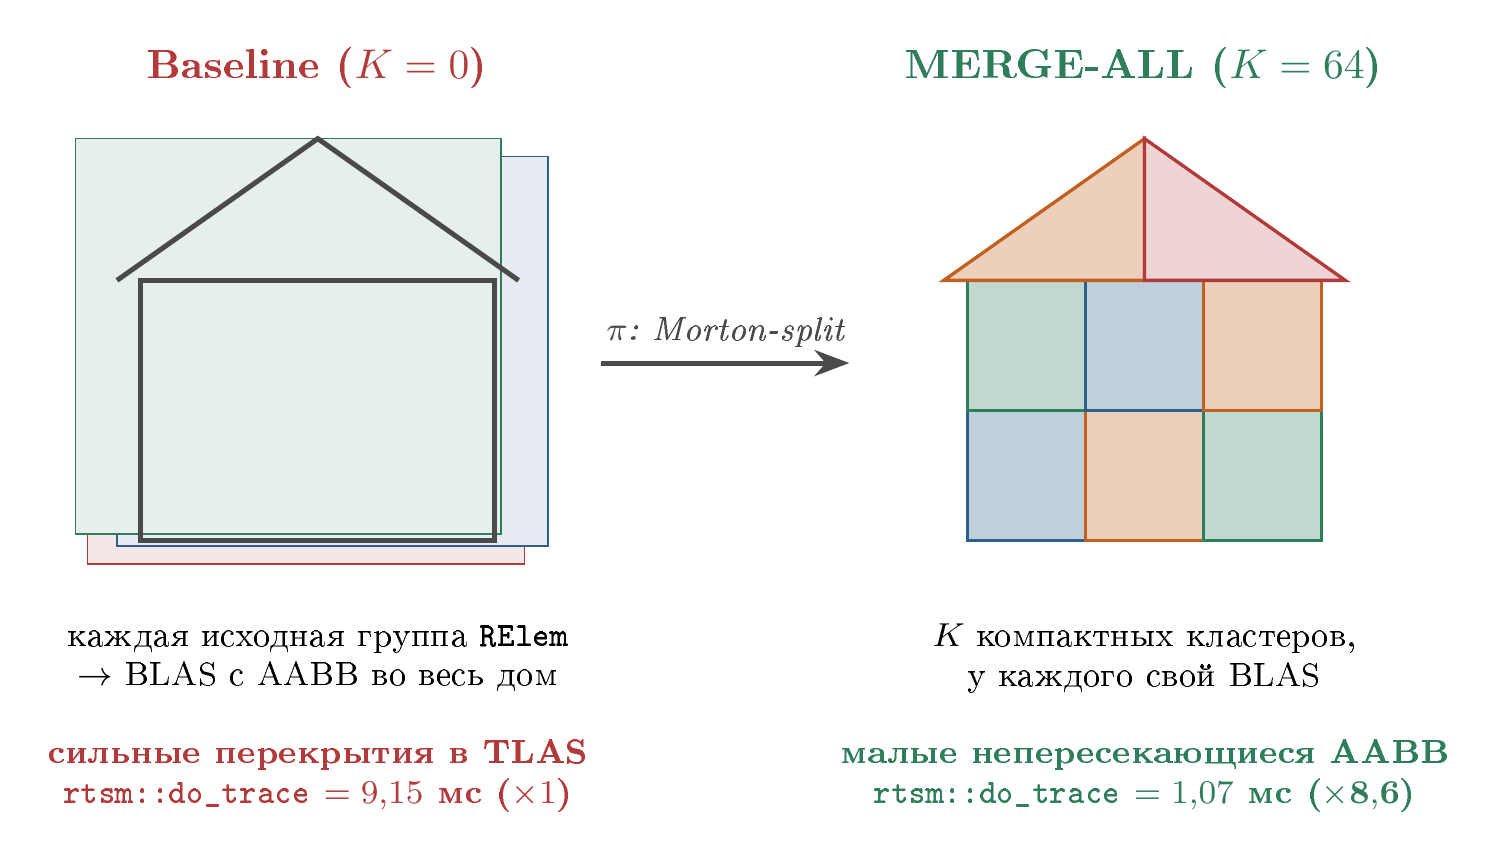
\includegraphics[width=0.8\textwidth]{diagrams/scheme_idea.png}
\caption{Идея метода. \textbf{Слева:} baseline --- каждая исходная
группа \texttt{RElem} даёт BLAS с AABB во весь дом, инстансы в TLAS
сильно перекрываются ($9{,}15$~мс на худшем, случайном разбиении).
\textbf{Справа:} после Morton-кластеризации дом разбит на $K$ компактных
кластеров с малыми непересекающимися AABB, и время падает до
$1{,}07$~мс ($\mathbf{\times 8{,}6}$).}
\label{fig:idea}
\end{figure}

В этой версии метода материальная атрибуция треугольников теряется
(все треугольники объединяются под унифицированный
ray-tracing-материал), что приемлемо для трассировки теней RTSM,
где материал в hit-shader-е не используется. Это ограничение
обсуждается в заключении.

\subsubsection{Шаги алгоритма}

Пусть исходная модель содержит $R$ \texttt{RElem}-ов с числом
треугольников $|T_1|, \ldots, |T_R|$; обозначим
$N\!=\!\sum_k |T_k|$ --- полное число треугольников модели.

\begin{enumerate}
    \item \textbf{Сбор треугольников.} Для каждого
      \texttt{RElem}-а через \texttt{lockVbufferEx} и
      \texttt{lockIbufferEx} прочитываются позиции вершин
      (формат \texttt{VSDT\_FLOAT3}) и индексы (формат
      \texttt{uint16\_t}). Из них формируется массив
      $\{(\mathbf{p}_0^i, \mathbf{p}_1^i, \mathbf{p}_2^i)\}_{i=1}^{N}$
      позиций треугольников в локальной системе модели.
    \item \textbf{Глобальный AABB и центроиды.} Здесь $t_i$ --- $i$-й
      треугольник модели (с вершинами $\mathbf{p}_0^i, \mathbf{p}_1^i,
      \mathbf{p}_2^i$ из шага 1), а $M$ --- вся модель, то есть
      объединение всех её треугольников $t_1,\ldots,t_N$. Вычисляется
      габаритный бокс всей модели как объединение боксов отдельных
      треугольников
      $\mathrm{AABB}(M)\!=\!\bigcup_i \mathrm{AABB}(t_i)$ и набор
      центроидов (центров масс) треугольников
      $\mathbf{c}_i = (\mathbf{p}_0^i+\mathbf{p}_1^i+\mathbf{p}_2^i)/3$.
      Эти величины --- подготовка к Morton-сортировке (шаг 3):
      $\mathrm{AABB}(M)$ задаёт диапазон нормировки координат в
      $[0,1]^3$, а центроиды $\mathbf{c}_i$ служат ключом сортировки
      треугольников по пространственной близости.
    \item \textbf{Morton-сортировка.} Для каждого центроида
      вычисляется 63-битный Morton-код:
      нормированные координаты $\hat{\mathbf{c}}_i \in [0,1]^3$
      квантуются в 21-битные целые $\mathbf{q}_i \in
      \{0,\ldots,2^{21}-1\}^3$, и биты перемежаются:
      \[
          \mu(\mathbf{c}_i) =
          \sum_{b=0}^{20}\!\Bigl(
              q_{i,x}^{(b)}\!\cdot\!2^{3b}
              + q_{i,y}^{(b)}\!\cdot\!2^{3b+1}
              + q_{i,z}^{(b)}\!\cdot\!2^{3b+2}
          \Bigr).
      \]
      Треугольники сортируются стабильно по убыванию приоритета
      $\mu$.
    \item \textbf{Согласование $K$ с лимитом 16-битного индекса.}
      Пусть пользовательский запрос на число кластеров --
      $K_{\text{req}}$ (параметр
      \texttt{bvhMergeAllRelems} в \texttt{settings.blk}).
      Эффективное число кластеров:
      \[
          K \;=\; \max\!\Bigl(K_{\text{req}},\
              \bigl\lceil N / T_{\max} \bigr\rceil\Bigr),
          \qquad T_{\max} = 21\,845.
      \]
      Условие $K \ge \lceil N/T_{\max} \rceil$ гарантирует, что
      ни один кластер не превысит лимит 16-битного индекса.
    \item \textbf{Разбиение и формирование BLAS-ов.}
      Отсортированный пул делится на $K$ последовательных
      сегментов размера $\sim N/K$. Для каждого сегмента $j$:
      \begin{itemize}
          \item выделяется собственный vertex-буфер $V_j$;
          \item выделяется собственный index-буфер $I_j$;
          \item index-буфер создаётся с флагами
            \texttt{SBCF\_BIND\_SHADER\_RES} и
            \texttt{SBCF\_MISC\_ALLOW\_RAW}; они нужны для
            обращения к буферу как к SRV в compute-шейдере
            \texttt{BVH::IndexProcessor};
          \item сегмент регистрируется через
            \texttt{bvh::add\_mesh()} с уникальным
            \texttt{mesh\_id}, образованным из идентификатора
            ресурса и индекса кластера.
      \end{itemize}
    \item \textbf{Размещение инстансов.} При вызове
      \texttt{bvh::add\_instance()} в TLAS добавляется $K$
      инстансов новых кластеров с общей матрицей трансформации
      экземпляра.
\end{enumerate}

Полный конвейер из шести шагов и его единственный управляющий
параметр сведены на схеме конвейера ниже.

\begin{figure}[h!]
\centering
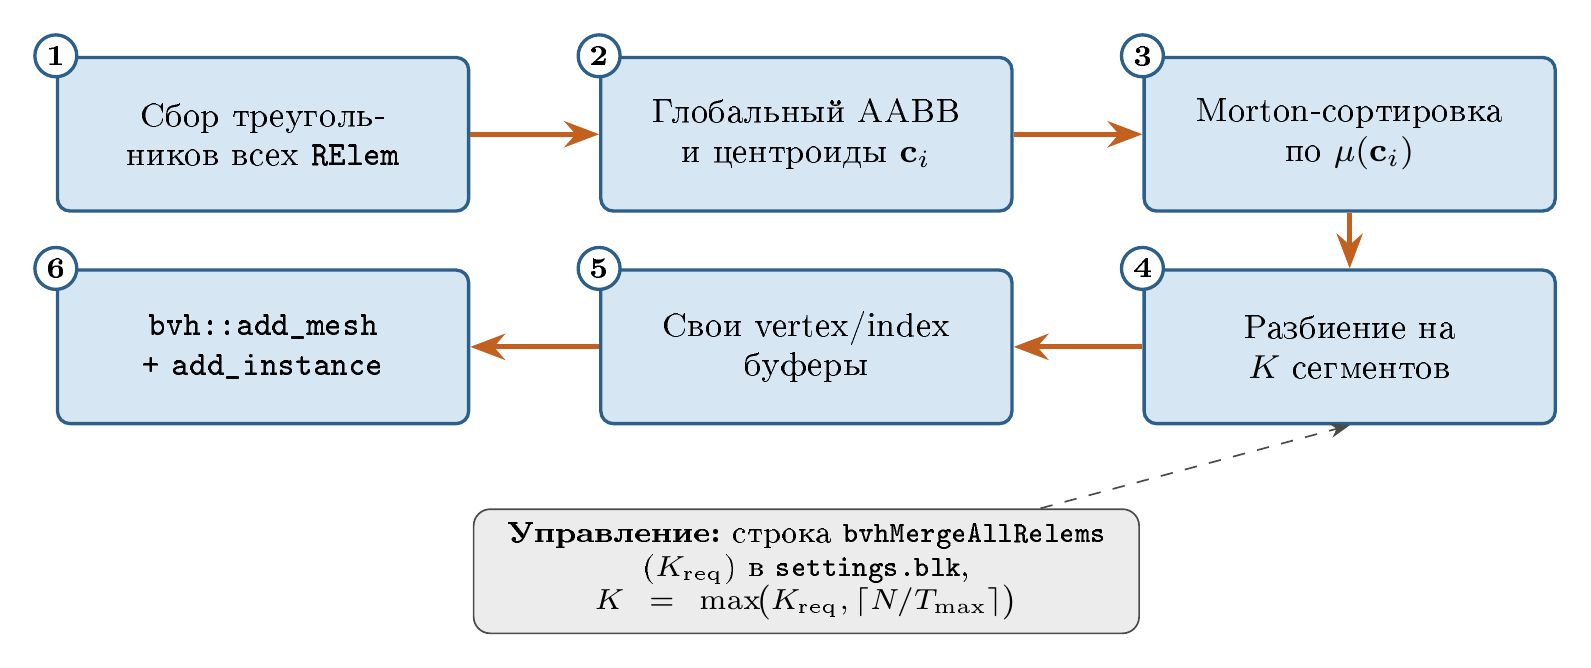
\includegraphics[width=0.85\textwidth]{diagrams/scheme_pipeline.png}
\caption{Конвейер метода: от сбора \texttt{RElem}-ов модели через
глобальную Morton-сортировку и разбиение на $K$ кластеров до регистрации
их в BVH. Управление --- одна строка \texttt{bvhMergeAllRelems} в
\texttt{settings.blk}; эффективное число кластеров согласуется с
аппаратным лимитом 16-битного индекса.}
\label{fig:pipeline}
\end{figure}

\subsubsection{Сложность}

Сбор треугольников и вычисление центроидов --- $O(N)$ при пиковой
памяти $O(N)$. Morton-сортировка стабильна и в реализации
основана на \texttt{eastl::sort}; в худшем случае
$O(N\log N)$. Формирование $K$ vertex/index-буферов и
регистрация --- $O(N)$. Итоговая асимптотика метода --
$O(N\log N)$, пиковая память $O(N)$. Алгоритм работает один раз
при инициализации BVH-контекста и не влияет на per-frame
стоимость рендера.

\subsubsection{Корректность}

\begin{enumerate}
    \item Множество треугольников не меняется. Каждый треугольник
      исходного меша попадает ровно в один кластер. Это
      обеспечивает покрытие сцены в трассировке.
    \item Позиции вершин копируются побитово (с приведением
      исходного формата к \texttt{Point3} при необходимости);
      визуальная эквивалентность теневой картинки следует из
      инвариантности набора треугольников.
    \item Автоматическое
      увеличение $K$ до $\lceil N/T_{\max}\rceil$ гарантируют
      работоспособность метода в рамках аппаратных ограничений
      DXR Tier 1.1.
\end{enumerate}

\subsection{Способ валидации}
\label{ssec:p3}

Улучшение качества BVH должно отражаться на реальной
производительности, иначе ценность метода сомнительна.
Поэтому валидация проводится в семпле \texttt{testGI} DagorEngine, который
рассчитан на нагрузочные эксперименты с рейтрейсингом и обладает
встроенным GPU-профайлером с per-pass таймингами.

\paragraph{Тестовая модель.} За основу взята общедоступная модель
жилого дома
\texttt{House, Ko Bulon Don Urak Lawoi Village, Thailand}. Для изоляции исследуемой проблемы и
проведения контролируемых тестов из неё подготовлены два варианта
разбиения на меш-ассеты:
\begin{itemize}
    \item \textbf{«Плохой» вариант} (случайный split): треугольники
      модели разбиты на группы \emph{случайным образом}, без учёта
      материала и положения в пространстве. В результате каждая группа
      равномерно «размазана» по всему объёму дома, и её \texttt{RElem}
      получает AABB размером со всю модель --- синтетический худший
      случай с максимальными перекрытиями в TLAS.
    \item \textbf{Реалистичный вариант} (материальный split):
      треугольники сгруппированы \emph{по материалам} (металлические
      детали дверей и сантехники в одной группе, дерево в другой,
      стекло в третьей, и т.\,д.), как это обычно делает пайплайн
      игрового движка. Материалы частично локализованы по частям
      здания, поэтому перекрытия AABB слабее, чем при случайном
      разбиении; этот вариант служит честной точкой сравнения,
      соответствующей реальным production-моделям и гипотезе работы.
\end{itemize}
Оба варианта содержат одно и то же множество треугольников и дают
попиксельно одинаковую картинку; при этом различается лишь группировка
треугольников по \texttt{RElem}-ам.

\paragraph{Тестовая сцена.} В сцену \texttt{testGI} размещены
$N\!=\!16$ инстансов модели \texttt{House, Ko Bulon Don Urak Lawoi Village, Thailand}, чтобы получить
заметную RT-нагрузку. Активна подсистема ray-traced shadow maps
для одного направленного источника света (солнце). Итоговый вид
сцены приведён на рисунке ниже.

\begin{figure}[h!]
\centering
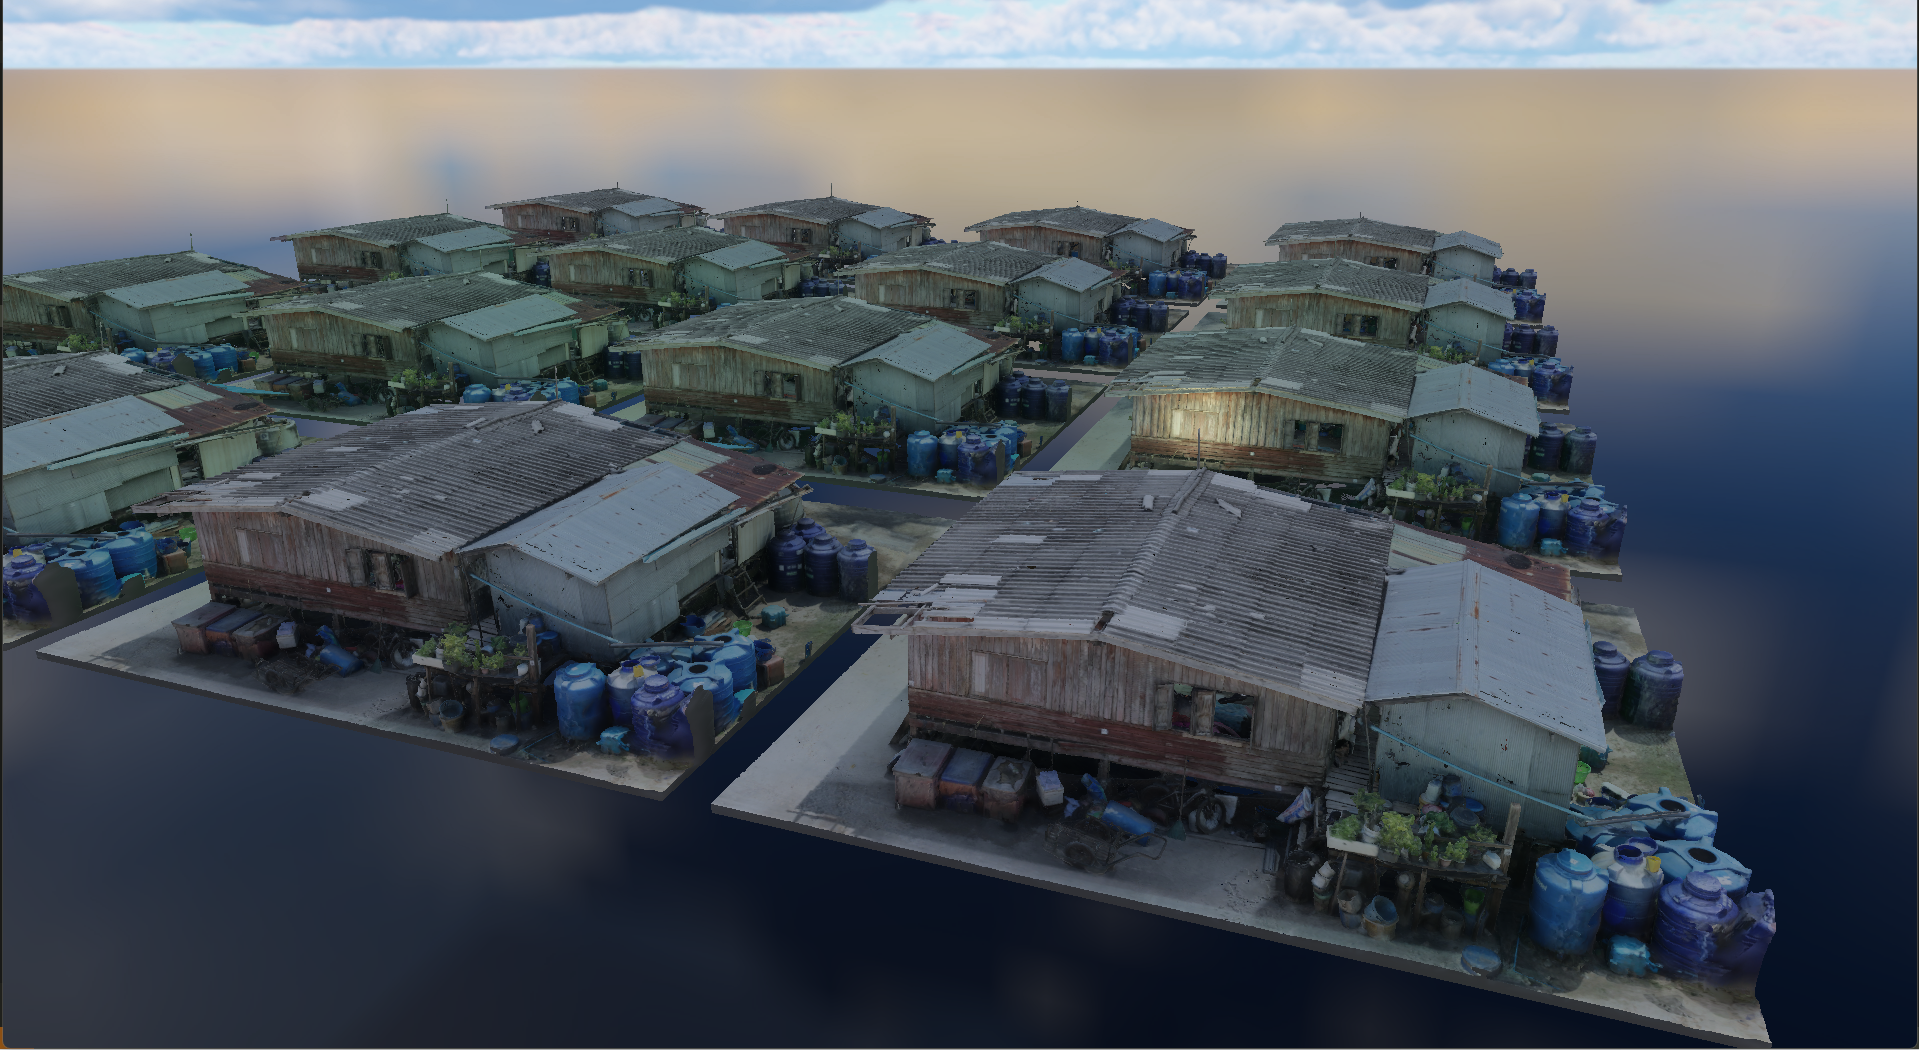
\includegraphics[width=0.78\textwidth]{scene.png}
\caption{Тестовая сцена в \texttt{testGI}: сетка $4\!\times\!4$ из
$16$ инстансов модели жилого дома с трассируемыми тенями от солнца. Именно на этой сцене
измеряется время прохода \texttt{rtsm::do\_trace}.}
\label{fig:scene_render}
\end{figure}

\paragraph{Замеряемая величина.} Медианное GPU-время прохода
\texttt{rtsm::do\_trace} из встроенного GPU-профайлера движка.
Замер выполняется в установившемся режиме (тёплый кэш
RTSM-денойзера, неподвижная камера, фиксированный кадровый
буфер).

\paragraph{Сравниваемые конфигурации.}
\begin{itemize}
    \item \textbf{Baseline.} Все опции оптимизации отключены
      (\texttt{bvhMergeAllRelems:i = 0}).
    \item \textbf{Глобальная пространственная кластеризация.} Включён
      \texttt{bvhMergeAllRelems:i = 64}: треугольники модели
      собираются, сортируются по Morton-коду центроида и
      разрезаются на не менее чем 64 пространственно-плотных
      кластеров.
\end{itemize}

\paragraph{Качественная валидация.} Дополнительно для оценки
качества пространственной локализации захватываются кадры в
Nsight~Graphics с раскраской BLAS-инстансов в режиме
\texttt{Color By: Instance}. На baseline-конфигурации ожидается
«шумовая» картина из перекрывающихся прямоугольников; на
оптимизированной --- крупные пространственно-связные области,
соответствующие отдельным BLAS-кластерам.

\subsection{Сводная схема предлагаемого решения}

Итоговое отображение $\pi$ задаётся следующей схемой:

\begin{equation*}
\bigl\{M_k\bigr\}_{k=1}^{R}
\;\xrightarrow[\text{Morton-сортировка}]{\text{объединение} + }\;
\bigl\{M'_j\bigr\}_{j=1}^{K}
\;\xrightarrow[\text{add\_mesh + add\_instance}]{\text{bvh::}}\;
\bigl\{T_j\bigr\}_{j=1}^{K},
\end{equation*}
\noindent
где $\{M_k\}_{k=1}^{R}$ --- исходные наборы треугольников модели
(материальные \texttt{RElem}-ы), $\{M'_j\}_{j=1}^{K}$ --
пространственно-компактные кластеры после объединения и
Morton-сортировки, а $\{T_j\}_{j=1}^{K}$ --- построенные драйвером
BLAS этих кластеров. Качество результата оценивается по медианному
GPU-времени \texttt{rtsm::do\_trace} в \texttt{testGI}
и качественной картиной Acceleration~Structure в Nsight~Graphics;
конкретные артефакты приведены в экспериментальной части.

\subsection{Параметры алгоритма и выбор значений}

Метод имеет один пользовательский параметр:
\textbf{$K_{\text{req}}$} (\texttt{bvhMergeAllRelems})~--- желаемое число
кластеров на модель. Для целевой модели \texttt{House}
($\sim 1{,}2$~млн треугольников) выбрано $K_{\text{req}}\!=\!64$ как
оптимум по результатам sweep в экспериментальной части.
Эффективное $K$ автоматически поднимается до
$\lceil N/T_{\max}\rceil\!=\!56$ при меньших запросах;
при $K_{\text{req}}\!\ge\!64$ используется запрошенное значение.

\subsection{Выводы по разделу}

Таким образом, задача декомпозирована на три подзадачи. Анализ
pipeline формирования BLAS выявил единственную доступную без модификации драйвера
точку вмешательства --- стадию
\texttt{RElem[]} и \texttt{RaytraceGeometryDescription[]}; на её
основе построен алгоритм глобальной пространственной кластеризации
со сложностью $O(N\log N)$ и сохранением множества треугольников по
построению; определён способ валидации --- прямой замер
\texttt{rtsm::do\_trace} в \texttt{testGI} и проверка локализации BLAS в
Nsight~Graphics. Метод и его единственный параметр $K_{\text{req}}$
готовы к экспериментальной проверке в практической части.
 %% Исследование и построение решения задачи
    \clearpage
    \section{Описание практической части}
\label{sec:Chapter4} \index{Chapter4}

Раздел документирует программную реализацию решения, разработанного
в предыдущей главе, и приводит результаты экспериментов.
Сначала описывается, куда именно в стек DagorEngine встроен метод,
затем --- детали алгоритмического модуля и, наконец, измеренное
ускорение трассировки. При этом все исходные коды, скрипты и сырые материалы
замеров размещены в репозитории работы~\cite{thesisRepo}.

Чтобы было понятно место метода в общей системе, ниже
приведён стек подсистем: от аппаратного
API DirectX~12 до измеряемого прохода \texttt{rtsm::do\_trace}.
В этом стеке предлагаемая предобработка вклинивается между подсистемой
\texttt{bvh} и вызовом построения BLAS.

\begin{figure}[h!]
\centering
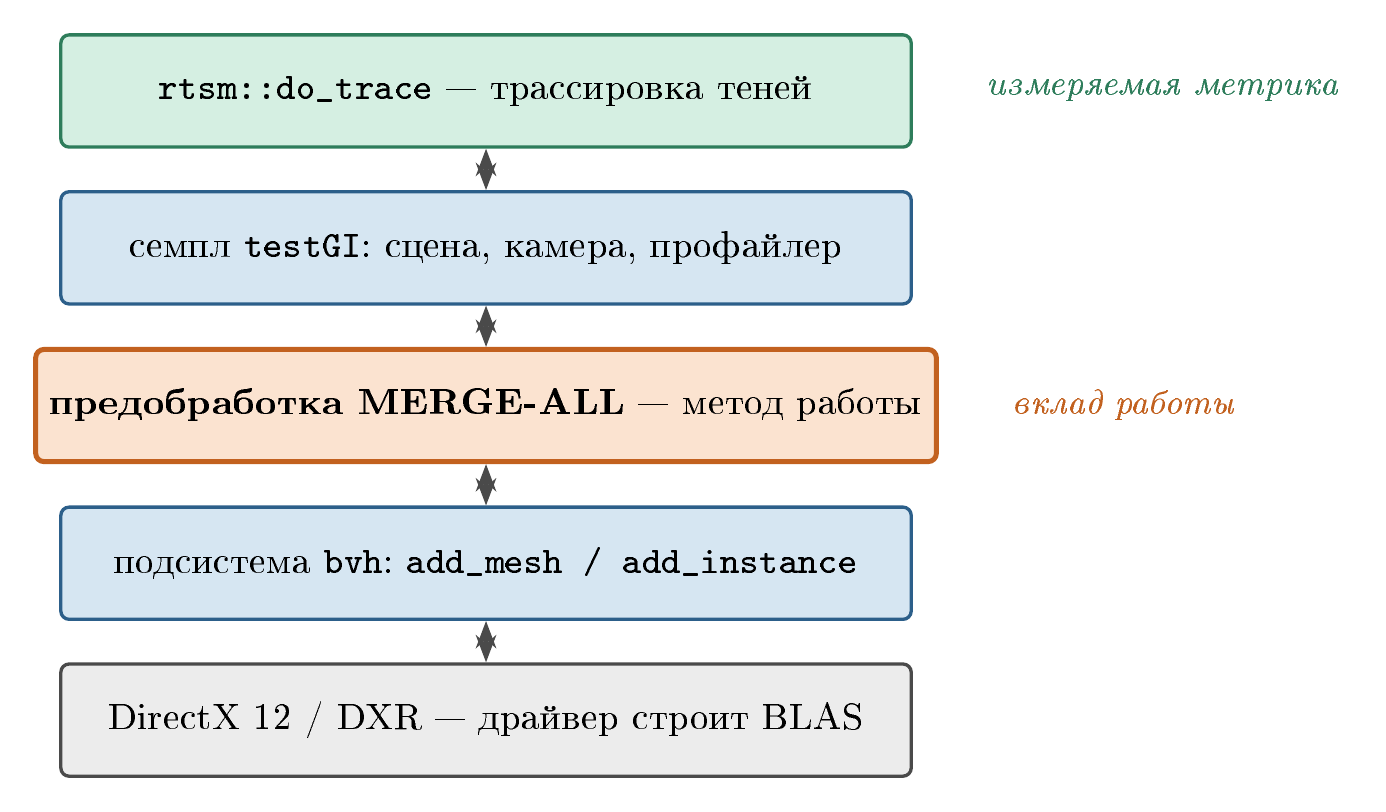
\includegraphics[width=0.68\textwidth]{diagrams/scheme_stack.png}
\caption{Стек подсистем: предобработка MERGE-ALL встроена на уровне
семпла \texttt{testGI} перед вызовами \texttt{bvh::add\_mesh} и не
требует изменений в драйвере или ассет-пайплайне. Измеряемая метрика ---
время верхнего прохода \texttt{rtsm::do\_trace}.}
\label{fig:stack}
\end{figure}

\subsection{Архитектура реализации}

Реализация локализована в семпле \texttt{testGI} движка
DagorEngine~\cite{dagorEngine} и состоит из двух частей:

\paragraph{(A) Алгоритмическая часть.} Код алгоритма вынесен в
namespace \texttt{testgi\_dynrend\_bvh\_pre}. Он расположен в файле
\texttt{samples/testGI/prog/test\_app.cpp} (около 600 строк
C++17). Реализация включает чтение треугольников из исходных
\texttt{ShaderMesh::RElem}, глобальную Morton-сортировку по
центроидам, разбиение на пространственно-плотные кластеры,
выделение для каждого кластера собственных vertex/index-буферов и
регистрация их в BVH-подсистеме движка через
\texttt{bvh::add\_mesh()} и \texttt{bvh::add\_instance()}.

\paragraph{(B) Конфигурационная часть.} Опция
\texttt{bvhMergeAllRelems} в файле
\texttt{samples/testGI/game/settings.blk} --- единственный
пользовательский управляющий параметр. Целочисленное значение
задаёт минимальное желаемое число пространственных кластеров на
модель; нулевое или отрицательное значение отключает метод и
возвращает поведение к baseline.

\subsection{Реализация алгоритмического модуля}

\subsubsection{Ключевые структуры данных}

\begin{verbatim}
struct SubMesh { uint32_t triStart, triCount; BSphere3 bsphere; };
struct MergedResourceState {
    uint32_t clusterCount;            // итоговое число кластеров K
    Tab<Sbuffer*> vbs, ibs;           // K vertex- и 16-bit index-буферов
};
struct ClusterRegistry {
    WinCritSec cs;
    eastl::vector_map<uint64_t, MergedResourceState> merged;
};
\end{verbatim}

\texttt{ClusterRegistry} живёт как singleton (ключ --- \texttt{bvh\_id}
ресурса); критическая секция обеспечивает потокобезопасность доступа
из BVH-обновлений.

\subsubsection{Основные функции}

\begin{itemize}
\item \texttt{gather\_relem\_triangles()} читает позиции
  треугольников одного \texttt{RElem}-а (формат \texttt{VSDT\_FLOAT3},
  16-битные индексы; RElem-ы с иным форматом пропускаются с
  предупреждением).
\item \texttt{try\_register\_merged\_resource()} --- основная
  функция: собирает глобальный пул треугольников всех \texttt{RElem}-ов,
  выполняет Morton-сортировку, согласует $K$ с лимитом 16-битного
  индекса, выделяет на каждый кластер свои vertex/index-буферы и
  регистрирует их через \texttt{bvh::add\_mesh()}.
\item \texttt{add\_dynrend\_resource\_to\_bvh()} и
  \texttt{add\_dynrend\_instance\_to\_bvh()} --- модифицированные
  точки входа: при $K\!>\!0$ стандартный per-\texttt{RElem} путь
  заменяется на $K$ кластеров/инстансов с общей трансформацией
  (уникальный 64-битный \texttt{mesh\_id} кодирует пару
  \texttt{(bvh\_id, cluster\_ix)}).
\end{itemize}

\subsubsection{Аппаратные требования к буферам}

Index-буферы кластеров создаются с явным набором флагов:
\begin{verbatim}
const uint32_t ibFlags = SBCF_BIND_INDEX
                       | SBCF_BIND_SHADER_RES
                       | SBCF_MISC_ALLOW_RAW;
Sbuffer *ib = d3d::create_ib(ibSize, ibFlags, "bvh_merged_ib");
\end{verbatim}

Флаги \texttt{SBCF\_BIND\_SHADER\_RES} и
\texttt{SBCF\_MISC\_ALLOW\_RAW} необходимы для того, чтобы
compute-шейдер \texttt{BVH::IndexProcessor} в Dagor мог
использовать буфер индексов как Shader~Resource~View. Без них
runtime срабатывает с \texttt{G\_ASSERT} в начале
BVH-постройки. Это требование выяснено эмпирически по дампам
крашей.

\subsubsection{Согласование $K$ с лимитом 16-битного индекса}

Реализация автоматически поднимает запрошенное $K_{req}$ до
минимально допустимого $K_{min}$. Для целевой модели (около $1{,}22 \cdot 10^6$
треугольников) при запросе \texttt{bvhMergeAllRelems:i = 16}
эффективное K=56 --- именно столько кластеров и регистрируется
(фиксируется в логе инициализации).

\subsection{Конфигурация семпла}

Единственный управляющий параметр --- строка
\texttt{bvhMergeAllRelems:i} в секции \texttt{graphics} файла
\texttt{samples/testGI/game/settings.blk} ($0$ --- метод отключён).
Опция читается при инициализации BVH-контекста и не требует
перезапуска приложения: смена значения вызывает штатный
\texttt{request\_full\_rebuild()}, как при смене RT-preset.

\subsection{Тестовый стенд}

\subsubsection{Сцена}

Сцена представляет собой $4\!\times\!4$ сетку из $N\!=\!16$
инстансов модели \texttt{House, Ko Bulon Don Urak Lawoi Village, Thailand} с шагом 15~м. Между моделями
оставлены проходы для имитации улицы; источник света --- одно
направленное солнце под наклоном $45^\circ$.

\subsubsection{Два варианта разбиения одной модели}

Эксперименты проводились на одной и той же геометрии дома в двух конфигурациях экспорта,
введённых в постановке задачи: \texttt{bad\_house} --- «плохой»
случайный split и
\texttt{bad\_house\_new\_mesh} --- реалистичный материальный split. Для каждого
варианта выполнена серия замеров при разных значениях
\texttt{bvhMergeAllRelems} ($K_{req}$) при фиксированной камере
и одинаковых настройках RTSM.

\subsubsection{Условия замера}

\defitem{Платформа}{Windows~11~x64, DirectX~12, GPU
  GeForce RTX-класса.}
\defitem{Семпл}{\texttt{testGI} из репозитория DagorEngine, сборка
  через штатный \texttt{jam}-скрипт.}
\defitem{Конфигурация}{\texttt{enableBVH=yes}, RTSM включён для
  солнечного источника, остальные RT-эффекты выключены.}
\defitem{Камера}{зафиксирована в одной позиции, обзор сетки
  инстансов под углом сверху-сбоку.}
\defitem{Замер}{медианное GPU-время GPU-маркера
  \texttt{rtsm::do\_trace} за 100 кадров после установления
  тёплого состояния денойзера.}
\defitem{Что не входит в замер}{время сборки BVH
  (\texttt{bvh::build}) и обновления TLAS --- эти операции
  происходят однократно при загрузке сцены и не влияют на
  per-frame стоимость.}

\subsection{Результаты}

\textbf{Главный результат:} предложенный метод снижает время
GPU-трассировки теней \texttt{rtsm::do\_trace} в \textbf{8{,}6 раза}
на синтетическом худшем разбиении (с 9,15 до 1,07~мс)
и в \textbf{2{,}7 раза} на реалистичном разбиении по материалам
(с 2,75 до 1,01~мс) --- при попиксельно идентичной картинке.
Оба результата превышают целевой критерий ($\ge\!2\times$). Ниже
этот результат разбирается подробно: сначала зависимость от числа кластеров
$K_{req}$, затем сводное сравнение и качественная картина
Acceleration~Structure.

\subsubsection{Зависимость времени трассировки от $K_{req}$}

Сводная таблица суммирует sweep по $K_{req}$ для
обоих вариантов разбиения. При $K_{req}$ не менее 64
эффективное число кластеров совпадает с запрошенным (лимит
16-битного индекса для данной модели --- $K_{min}$=56).

\begin{table}[h!]
\centering
\caption{Зависимость \texttt{rtsm::do\_trace} от $K_{req}$ для двух вариантов разбиения модели}
\label{tab:k_sweep}
\small
\begin{tabular}{r|rr|rr}
\hline
& \multicolumn{2}{c|}{\textbf{Случайный split}} &
  \multicolumn{2}{c}{\textbf{Материальный split}} \\
$K_{req}$ &
  \textbf{мс} & \textbf{ускор.} &
  \textbf{мс} & \textbf{ускор.} \\
\hline
0 (baseline) & 9{,}15 & \aptimes{1{,}0} & 2{,}75 & \aptimes{1{,}0} \\
64           & 1{,}07 & \aptimes{8{,}6} & 1{,}01 & \aptimes{2{,}7} \\
96           & 1{,}13 & \aptimes{8{,}1} & 1{,}06 & \aptimes{2{,}6} \\
128          & 1{,}22 & \aptimes{7{,}5} & 1{,}06 & \aptimes{2{,}6} \\
192          & 1{,}23 & \aptimes{7{,}4} & 1{,}11 & \aptimes{2{,}5} \\
256          & 1{,}30 & \aptimes{7{,}0} & 1{,}18 & \aptimes{2{,}3} \\
\hline
\end{tabular}
\end{table}

На «плохом» разбиении метод даёт до \textbf{8{,}6-кратного}
ускорения при $K_{req}$=64: baseline $9{,}15$~мс
против $1{,}07$~мс. На реалистичном разбиении baseline
уже ниже ($2{,}75$~мс), но Morton-кластеризация всё равно снижает
время до $1{,}01$~мс (\aptimes{2{,}7}). В обоих случаях наблюдается
плато $K_{req}$=64…128 и ухудшение при
$K_{req}$=256 из-за роста числа BLAS-инстансов в TLAS
($16$ моделей $\times$ $K$ кластеров). Эта зависимость наглядно
видна на графике ниже.

\begin{figure}[H]
\centering
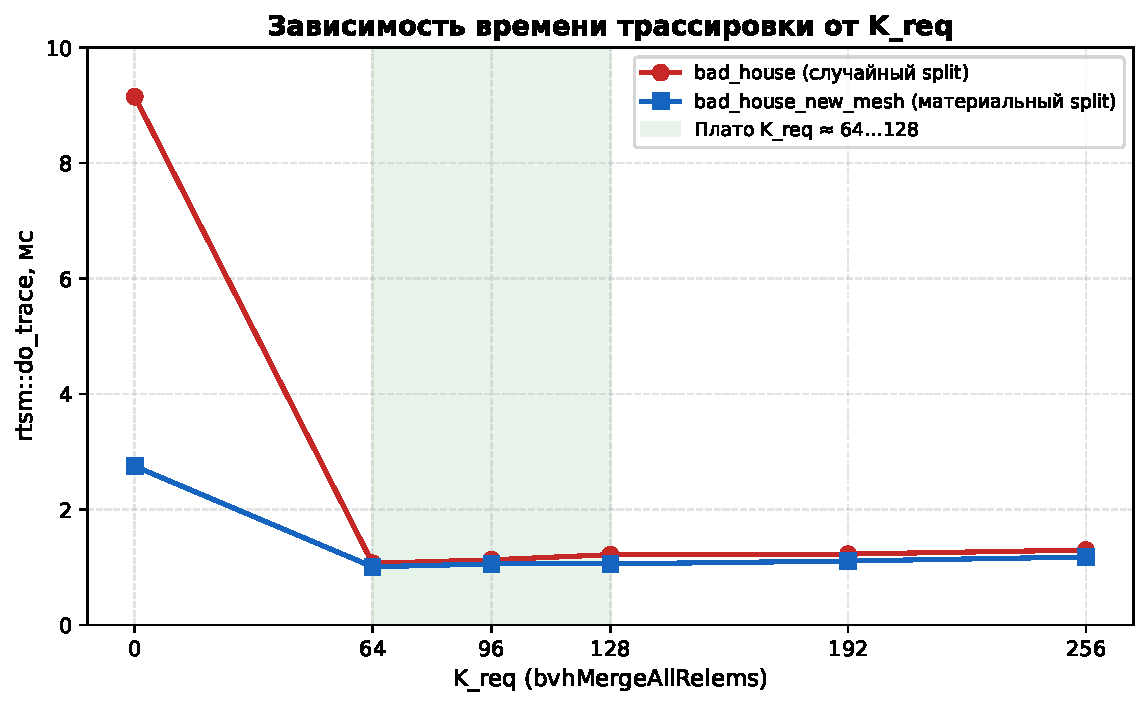
\includegraphics[width=0.78\textwidth]{diagrams/05_k_sweep_chart.pdf}
\caption{Зависимость времени \texttt{rtsm::do\_trace} от запрошенного
числа кластеров $K_{req}$ для двух вариантов разбиения модели.}
\label{fig:k_sweep}
\end{figure}

\subsubsection{Сводное сравнение baseline и оптимума}

\begin{table}[h!]
\centering
\caption{Baseline и оптимальная конфигурация
($K_{req}$=64) для двух вариантов разбиения}
\label{tab:rtsm_runtime}
\small
\begin{tabular}{lrrr}
\hline
\textbf{Вариант модели} &
  \textbf{baseline, мс} &
  \textbf{$K_{req}$=64, мс} &
  \textbf{Ускорение} \\
\hline
Случайный split (\texttt{bad\_house}) &
  9{,}15 & 1{,}07 & \aptimes{8{,}6} \\
Материальный split (\texttt{bad\_house\_new\_mesh}) &
  2{,}75 & 1{,}01 & \aptimes{2{,}7} \\
\hline
\end{tabular}
\end{table}

Метод даёт наибольший выигрыш там, где исходное разбиение создаёт
сильные перекрытия AABB в TLAS; на реалистичном
разбиении этот эффект меньше (\aptimes{2{,}7}), но остаётся значимым, а оптимум
$K_{req}$ тот же.

\subsubsection{Качественная картина Acceleration Structure}

На рисунках ниже
приведены захваты Acceleration~Structure из Nsight~Graphics
(режим \texttt{Color By: Instance}, каждый цвет --- отдельный
BLAS-инстанс).

\begin{figure}[H]
\centering
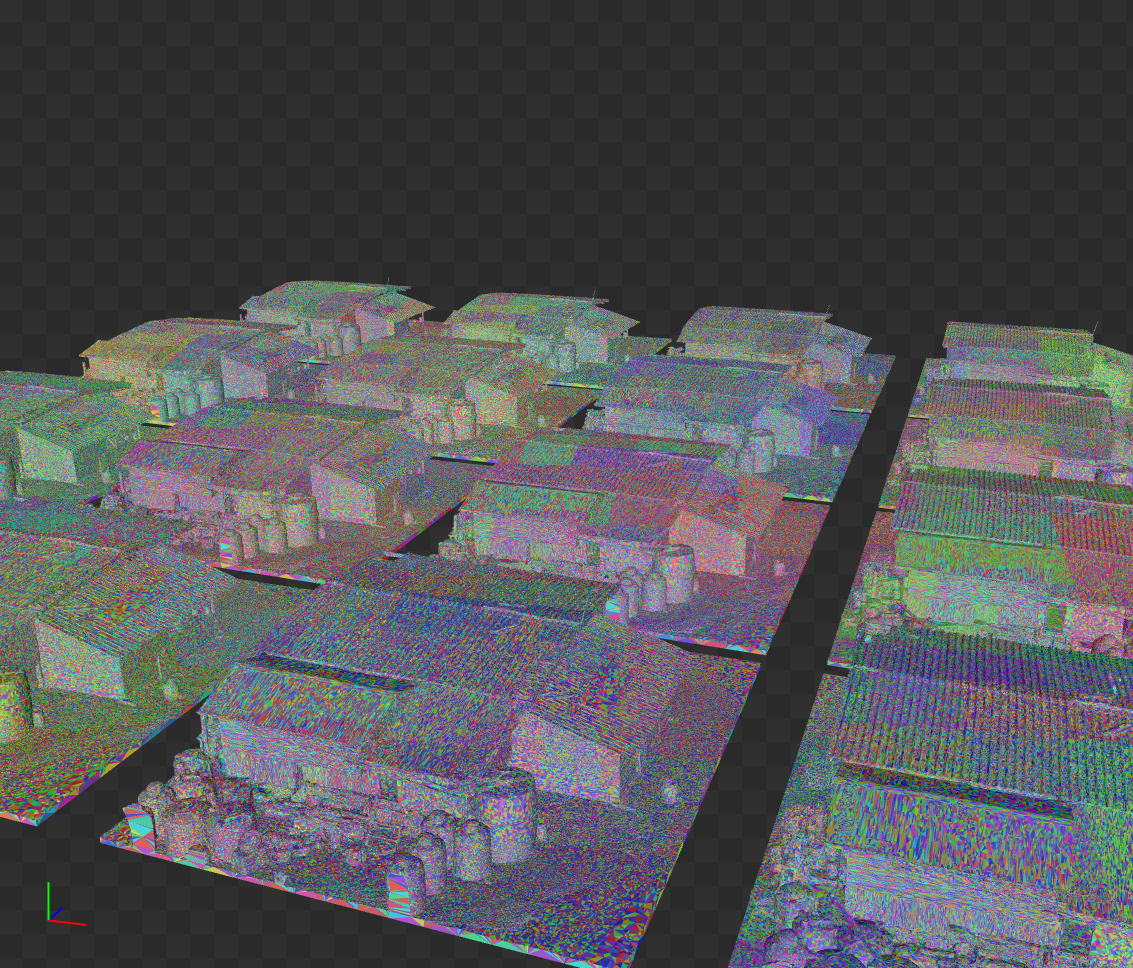
\includegraphics[width=0.72\textwidth]{no_optimized.png}
\caption{Случайный split. Наблюдается «шумовая»
картина из перекрывающихся BLAS-инстансов: на любой точке экрана
проецируется множество разных BLAS. Медианное \texttt{rtsm::do\_trace} = \textbf{9{,}15~мс}.}
\label{fig:dagor_with}
\end{figure}

\begin{figure}[H]
\centering
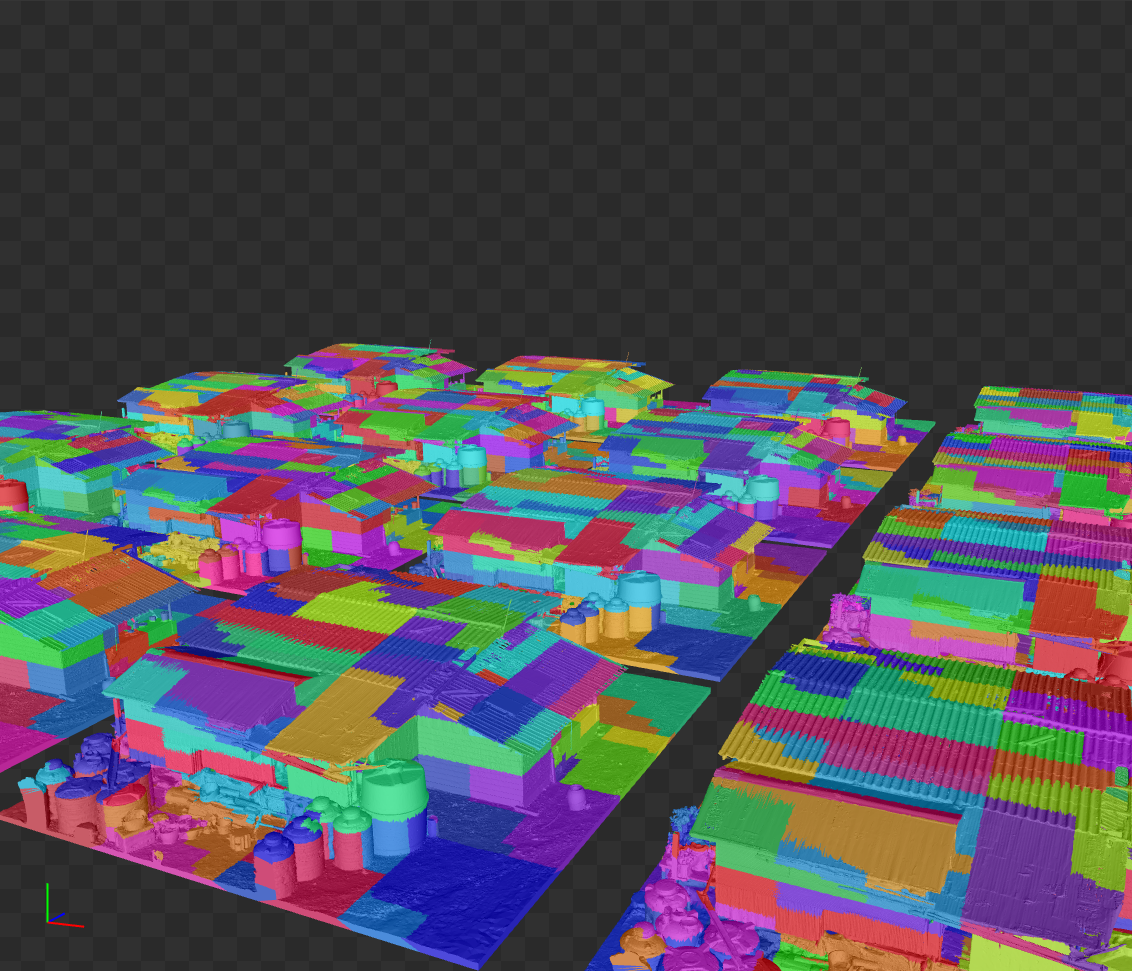
\includegraphics[width=0.72\textwidth]{with_optimization.png}
\caption{После применения метода.
Вместо шума отчётливо видны крупные сплошные цветные пятна --
каждый цвет соответствует одному пространственно-плотному
BLAS-кластеру. В каждом пикселе конкурируют 1--2 BLAS вместо
десятков. \texttt{rtsm::do\_trace} = \textbf{1{,}07~мс}.}
\label{fig:dagor_without}
\end{figure}

Визуальное сравнение подтверждает, что ускорение на «плохом»
разбиении обусловлено именно увеличением пространственной
локальности BLAS-инстансов, а не побочным эффектом подсистемы
RTSM.

Для контраста на отдельном рисунке показан тот же реалистичный
материальный split в исходном состоянии:
модель вручную разбита на группы по материалам, и каждый материал уже 
занимает сравнительно компактную область. Поэтому ещё до применения
метода Acceleration~Structure выглядит локализованной --- мелкие
пространственно-связные цветные пятна, а не сплошной «шум»
перекрывающихся инстансов. Именно это объясняет существенно меньшее
baseline-время на данном варианте ($2{,}75$~мс против $9{,}15$~мс на
случайном split) и более скромный, но устойчивый выигрыш метода
(\aptimes{2{,}7}).

\begin{figure}[H]
\centering
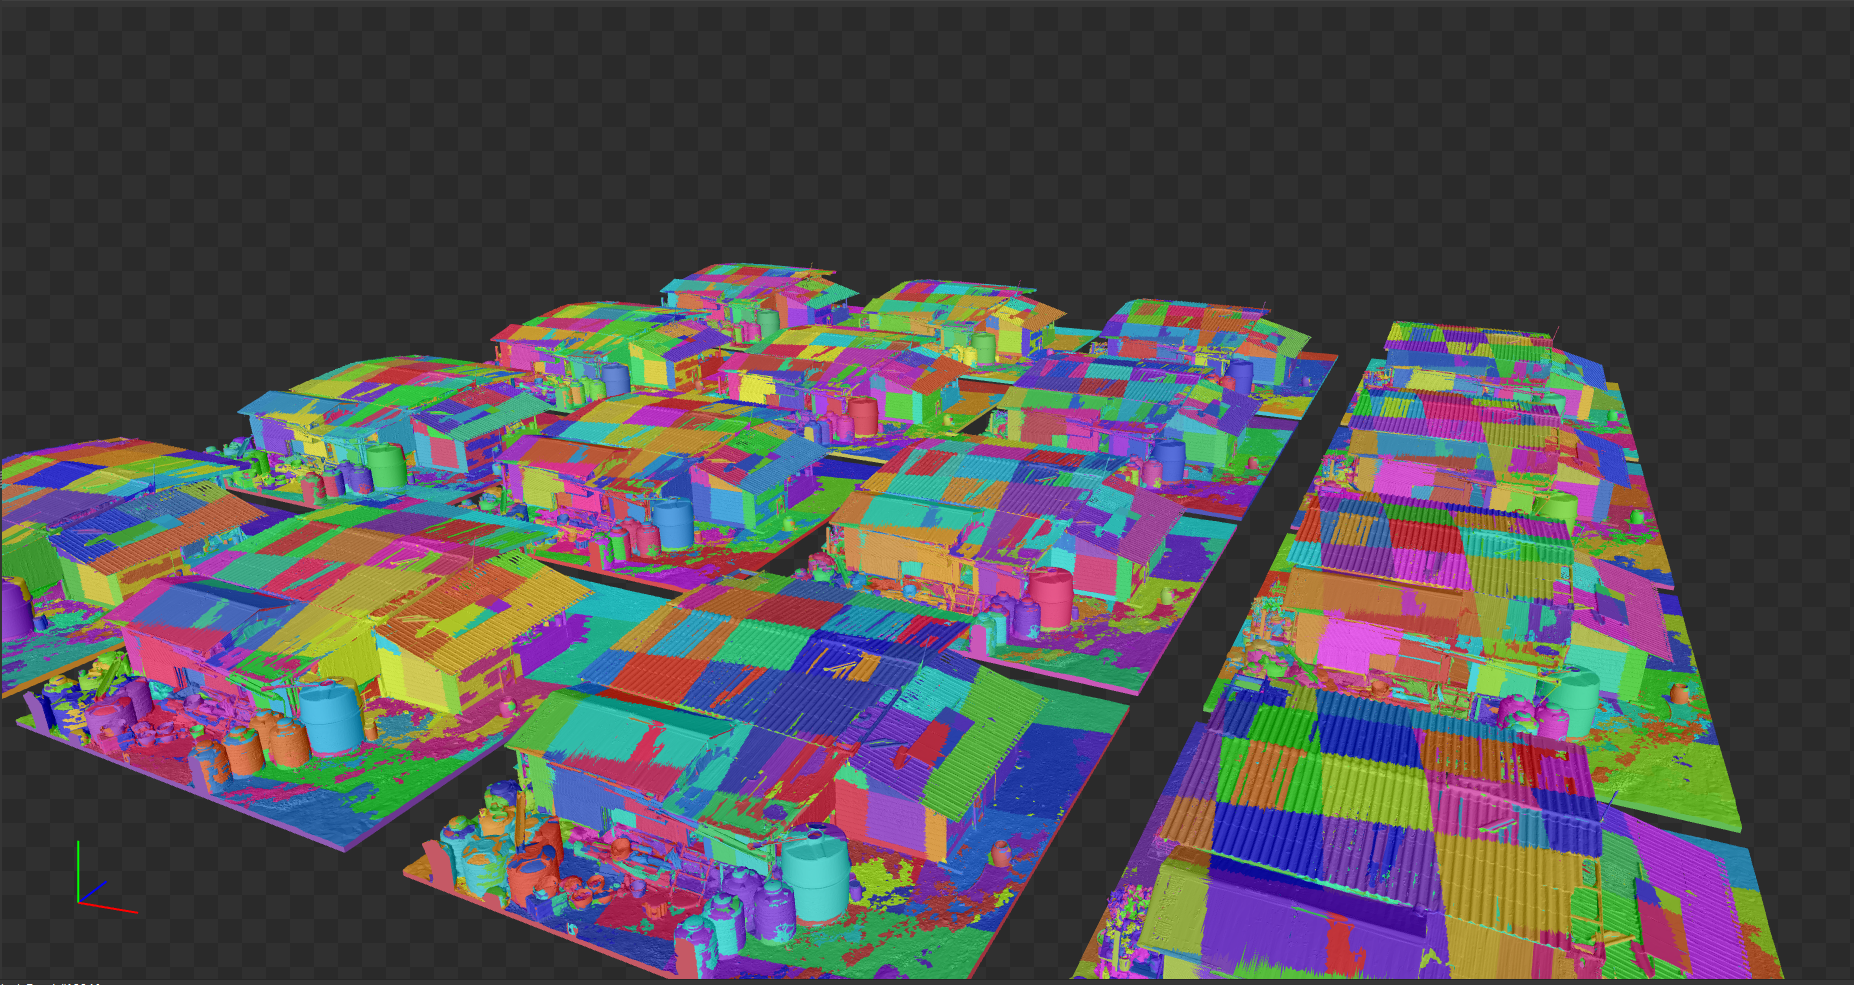
\includegraphics[width=0.72\textwidth]{real_mesh.png}
\caption{Реалистичный материальный split в исходном состоянии. Каждый цвет --- отдельный
материальный BLAS-инстанс. В отличие от случайного split, материалы уже
занимают сравнительно компактные области, поэтому картина выглядит
локализованной ещё \emph{до} применения метода. Медианное
\texttt{rtsm::do\_trace} = \textbf{2{,}75~мс}.}
\label{fig:real_mesh}
\end{figure}

\subsubsection{Выбор $K_{req}$}

Проход по сводной таблице показывает, что при
$K_{req}$=64 достигается минимальное время
\texttt{rtsm::do\_trace} для обоих вариантов модели.
Дальнейший рост~$K$ не улучшает результат: на
$K_{req}$=256 время растёт до $1{,}30$~мс (случайный
split) и $1{,}18$~мс (материальный split) --- накладные расходы
TLAS-обхода начинают доминировать над выигрышем от более мелких
AABB.

\subsection{Обсуждение}

\subsubsection{Интерпретация ускорения}

8{,}6-кратное ускорение на случайном split объясняется через
SAH-стоимость TLAS. В
baseline-конфигурации \texttt{bad\_house} каждая случайная группа
«размазана» по всей площади дома, её \texttt{RElem} образует BLAS с
AABB размером со всю модель, и при 16 инстансах TLAS заполняется
огромными перекрывающимися листьями. Любой луч проверяет пересечение с
большинством этих кандидатов, доля «полезной работы» мала из-за ложных пересечений с AABB --- это синтетический худший
случай, задающий верхнюю границу эффекта.

На реалистичном материальном split baseline уже составляет $2{,}75$~мс:
треугольники частично локализованы по материалам, перекрытия AABB
слабее, и выигрыш меньше (\aptimes{2{,}7}). Именно этот вариант
соответствует реальному пайплайну движка и напрямую подтверждает
гипотезу работы.

После применения метода с $K_{req}$=64 ассет разбивается
на $64$ пространственно-компактных кластера. В TLAS для всей сцены
присутствует $16 \times 64 = 1024$ TLAS-инстансов, ссылающихся на 64 уникальных BLAS, но каждый из инстансов имеет малый AABB,
слабо перекрывающий соседей. Алгоритм обхода TLAS быстро отбрасывает
нерелевантные ветви; при этом при $K_{req}$=256 перекрытия уже
не доминируют, и накладные расходы обхода большого TLAS снова растут.

\subsubsection{Цена ускорения}

Метод увеличивает число BLAS-инстансов на одну модель с
$R \approx 10$ (исходные \texttt{RElem}-ы) до
$K_{req}$ (при оптимуме $K_{req}$=64 --- до
$64$ кластеров). Дополнительный объём памяти на vertex/index-буферы
кластеров составляет $\sim 30$~Мб для всей сцены из 16
инстансов; объём BLAS-узлов растёт пропорционально числу
BLAS-инстансов. Время одноразовой инициализации
(\texttt{bvh::build}) увеличивается на десятки миллисекунд за
счёт большего числа BLAS-построек, но per-frame стоимость
\texttt{rtsm::do\_trace} на «плохом» split падает более чем
в $8$ раз --- что и является целью.

\subsubsection{Ограничения текущей реализации}

Метод имеет ряд ограничений: он теряет per-triangle материальную
атрибуцию, работает только с основным уровнем
детализации, требует ручного выбора $K_{req}$ и неприменим к
анимированным ассетам (скелет, морф-таргеты), вершины которых меняются
каждый кадр. Пути их снятия рассмотрены в заключении.
 %% Описание практической части
    \clearpage
    \section{Заключение}
\label{sec:Chapter5} \index{Chapter5}

\subsection{Решённая задача}

В работе исследована проблема качества Bottom-Level Acceleration
Structure, построенной вендорским DXR/Vulkan-билдером по входным
данным современного игрового движка. На основе этого сформулирована и
экспериментально проверена гипотеза о том, что выделение отдельного BLAS под каждую материальную подгруппу, разбросанную по всему объёму модели, порождает огромные BLAS-инстансы,
которые создают сильные перекрытия в структуре верхнего уровня,
что может существенно ухудшать время трассировки лучей. Эта гипотеза, выдвинутая на основе
эмпирических наблюдений на сценах
DagorEngine, получила в данной работе
\emph{количественное} подтверждение: на реалистичном разбиении модели
по материалам реализация предложенного метода даёт снижение времени
трассировки теней в $2{,}7$ раза, а на синтетическом худшем
разбиении --- до $8{,}6$ раза.

\subsection{Полученные результаты}

\begin{enumerate}
    \item Описана полная цепочка преобразований
      от ресурса модели до массива \texttt{RaytraceGeometryDescription[]}
      и итогового BLAS в DagorEngine. Идентифицирована доступная точка
      разработческого вмешательства, совместимая с контрактом DXR --
      стадия формирования \texttt{RElem}-массива перед вызовом
      \texttt{bvh::add\_mesh()}.
    \item Разработан алгоритм глобальной пространственной кластеризации:
      объединение треугольников всех \texttt{RElem}-ов модели,
      глобальная Morton-сортировка по центроидам, разбиение на
      пространственно-плотные кластеры с автоматической
      корректировкой их числа под аппаратный лимит 16-битного
      индекса. Линейно-логарифмическая сложность $O(N\log N)$,
      пиковая память $O(N)$, корректность доказана по построению.
    \item Реализация выполнена в семпле \texttt{testGI} движка
      DagorEngine. Код алгоритма расположен в
      \texttt{test\_app.cpp}, а управление вынесено в опцию
      \texttt{bvhMergeAllRelems}. Метод встраивается как hook
      перед штатными вызовами BVH-подсистемы и не требует
      модификации ассет-пайплайна.
    \item На целевой сцене из 16 инстансов модели метод даёт до $8{,}6$-кратного ускорения основного
      прохода GPU-трассировки теней на синтетическом случайном split:
      \texttt{rtsm::do\_trace} снижается с $9{,}15$~мс до $1{,}07$~мс; на реалистичном материальном split ---
      \aptimes{2{,}7} (с 2,75 до 1,01~мс).
    \item Визуальное подтверждение --- захваты
      Acceleration-Structure в Nsight~Graphics. В режиме раскраски
      по инстансам вместо «шумовой» картины перекрывающихся
      BLAS-инстансов появляются крупные пространственно-связные
      цветные области, соответствующие отдельным BLAS-кластерам.
\end{enumerate}

\subsection{Соответствие критериям приёмки}

В постановке задачи сформулирован
набор формальных критериев; ниже приведено их соответствие выполненной работе:

\begin{enumerate}
    \item Реализован метод как опциональный режим инициализации
      BVH-контекста, включаемый одной строкой в
      \texttt{settings.blk} и собирающийся штатным
      jam-скриптом DagorEngine. \textbf{Выполнено.}
    \item На целевой сцене зафиксировано ускорение
      до \aptimes{8{,}6} на худшем случае и \aptimes{2{,}7} на реалистичном случае против критерия не менее \aptimes{2}.
      \textbf{Выполнено.}
    \item Визуальная картина Acceleration~Structure
      демонстрирует пространственно-связные области,
      подтверждая работу алгоритма. \textbf{Выполнено.}
    \item Тени до и после применения метода визуально
      неотличимы; множество треугольников сохраняется по
      построению. \textbf{Выполнено по построению.}
\end{enumerate}

\subsection{Научная новизна и практическая значимость}

\textbf{Научная новизна} работы заключается в следующих
результатах:
\begin{itemize}
    \item Формализована проблема деградации TLAS: разбросанные по объёму модели элементы одного материала порождают огромные BLAS, которые при сборке TLAS образуют сильно перекрывающиеся листовые узлы, приводя к огромному числу ложных пересечений и резкому падению производительности.
    \item Предложен метод глобальной пространственной кластеризации ассетов,
      занимающий уникальную нишу:
      \emph{вход билдера + DXR-совместимость + сохранение
      визуальной эквивалентности} (см.
      сводную таблицу сравнения подходов). Существующие подходы либо
      работают внутри билдера (HLBVH, SBVH), либо разрезают
      отдельные треугольники без учёта поэлементной структуры
      ассета (Ganestam-Doggett).
    \item Эффективность метода продемонстрирована
      \emph{не на симуляторе и не на офлайн-метрике}, а через
      реальный замер GPU-времени в работающем семпле
      production-движка. Восьмикратное снижение
      \texttt{rtsm::do\_trace} --- редкий по величине эффект для
      одной локальной оптимизации, что подтверждает существенное
      влияние проблемы пространственной локализации в DXR-BVH.
\end{itemize}

\textbf{Практическая значимость}: метод применяется как
runtime-опция инициализации BVH-контекста для динамических
ассетов и интегрируется в существующий код движка без изменения
формата хранения мешей. Это делает его пригодным для применения
в production-проектах, использующих большие массивы готовых
ассетов, в которых перезапекание невозможно или слишком дорого.

\subsection{Направления дальнейшего развития}

\begin{enumerate}
    \item \textbf{Сохранение материальной атрибуции.} Текущая
      реализация теряет материальный идентификатор отдельных
      треугольников, что приемлемо для трассировки теней RTSM,
      но не для подсистем, использующих hit-shader (отражения). Решение: для каждого кластера хранить
      side-buffer с соответствием «локальный треугольник --- материал»
      и обращаться к нему из hit-shader-а через
      индекс вклада инстанса в DXR.
    \item \textbf{Автоматический подбор $K$.} Текущее значение
      $K$ задаётся вручную в~\texttt{settings.blk}.
      Эвристика подбора по характеристикам модели (число
      треугольников, диагональ AABB, отношение AABB к
      пространству сцены) позволит избежать ручной настройки
      под каждую модель.
    \item \textbf{Альтернативные стратегии кластеризации.}
      Глобальная Morton-кластеризация --- простой и хорошо
      работающий baseline. На моделях с сильно неоднородным
      распределением треугольников более эффективными могут
      оказаться k-means по центроидам или octree-кластеризация
      с учётом SAH-cost внутри кластера.
    \item \textbf{Полная интеграция в ассет-пайплайн.} Текущая
      реализация выполняет split каждый раз при инициализации
      BVH-контекста; для production-проектов целесообразно
      перенести Morton-сортировку и разбиение в офлайн-стадию
      запекания ассета.
    \item \textbf{Валидация на дополнительных сценах.} Текущий
      результат получен на одной целевой сцене с одной моделью.
      Расширение замеров на production-сцены DagorEngine
      позволит оценить применимость метода в
      реальных условиях и на более сложных наборах данных.
\end{enumerate}

\subsection{Итог}

Поставленная задача --- разработать и экспериментально оценить
метод предобработки меша, повышающий качество BLAS, построенного
вендорским билдером, без модификации драйвера и с измеримым
ускорением реальной GPU-трассировки --- решена. В результате разработанный
алгоритм глобальной пространственной кластеризации, его реализация в
семпле \texttt{testGI} DagorEngine и проведённые замеры образуют
законченный набор результатов для дальнейшего исследования и
переноса метода в production-окружение.

Все исходные коды реализации, тестовая модель, скриншоты
Nsight-захватов и сопровождающие материалы опубликованы в
репозитории работы~\cite{thesisRepo}.
 %% Заключение
    \clearpage

    %% НЕ ТРОГАЙТЕ!!!
    \nocite{*}
    \sloppy
    \bibliography{references}
    \fussy

    %% в зависимости от надобности подключаем раздел "Приложение"
    % \newpage
    % \input{Appendix.tex}
\end{document}
